\graphicspath{{DistributionAnalysis/Figures/}}

\chapter{Distribution Analysis} \label{sec: disanalysis}

\section{Normalized Distributions}\label{sec: Normalized Distributions}

The normalized plots are useful to check the shape of backgrounds and signal distributions. These shapes help to identify which variables are not useful for the analysis because the backgrounds overlap with the signal and which variables have to be studied with greater detail because the signal separates from the backgrounds from certain points. An example for both cases is provided in Figures \ref{fig: tau2etaunitNC} and \ref{fig: tau1ptunitNC}. In figure \ref{fig: tau2etaunitNC} it can be seen that the signal overlaps for all values with the background distributions. That is why this plot can be used to conclude that the $\eta$ variable from the sub-leading $\tau$ is not useful to isolate the signal from the background. In contrast, the plot in Figure \ref{fig: tau1ptunitNC} show that from around 150 GeV the signal separates from the background distributions. This separation for the $p_{T}$ of the leading $\tau$ suggests that this variable should be examined more closely through the subsequent cuts. 

\begin{figure}
\centering
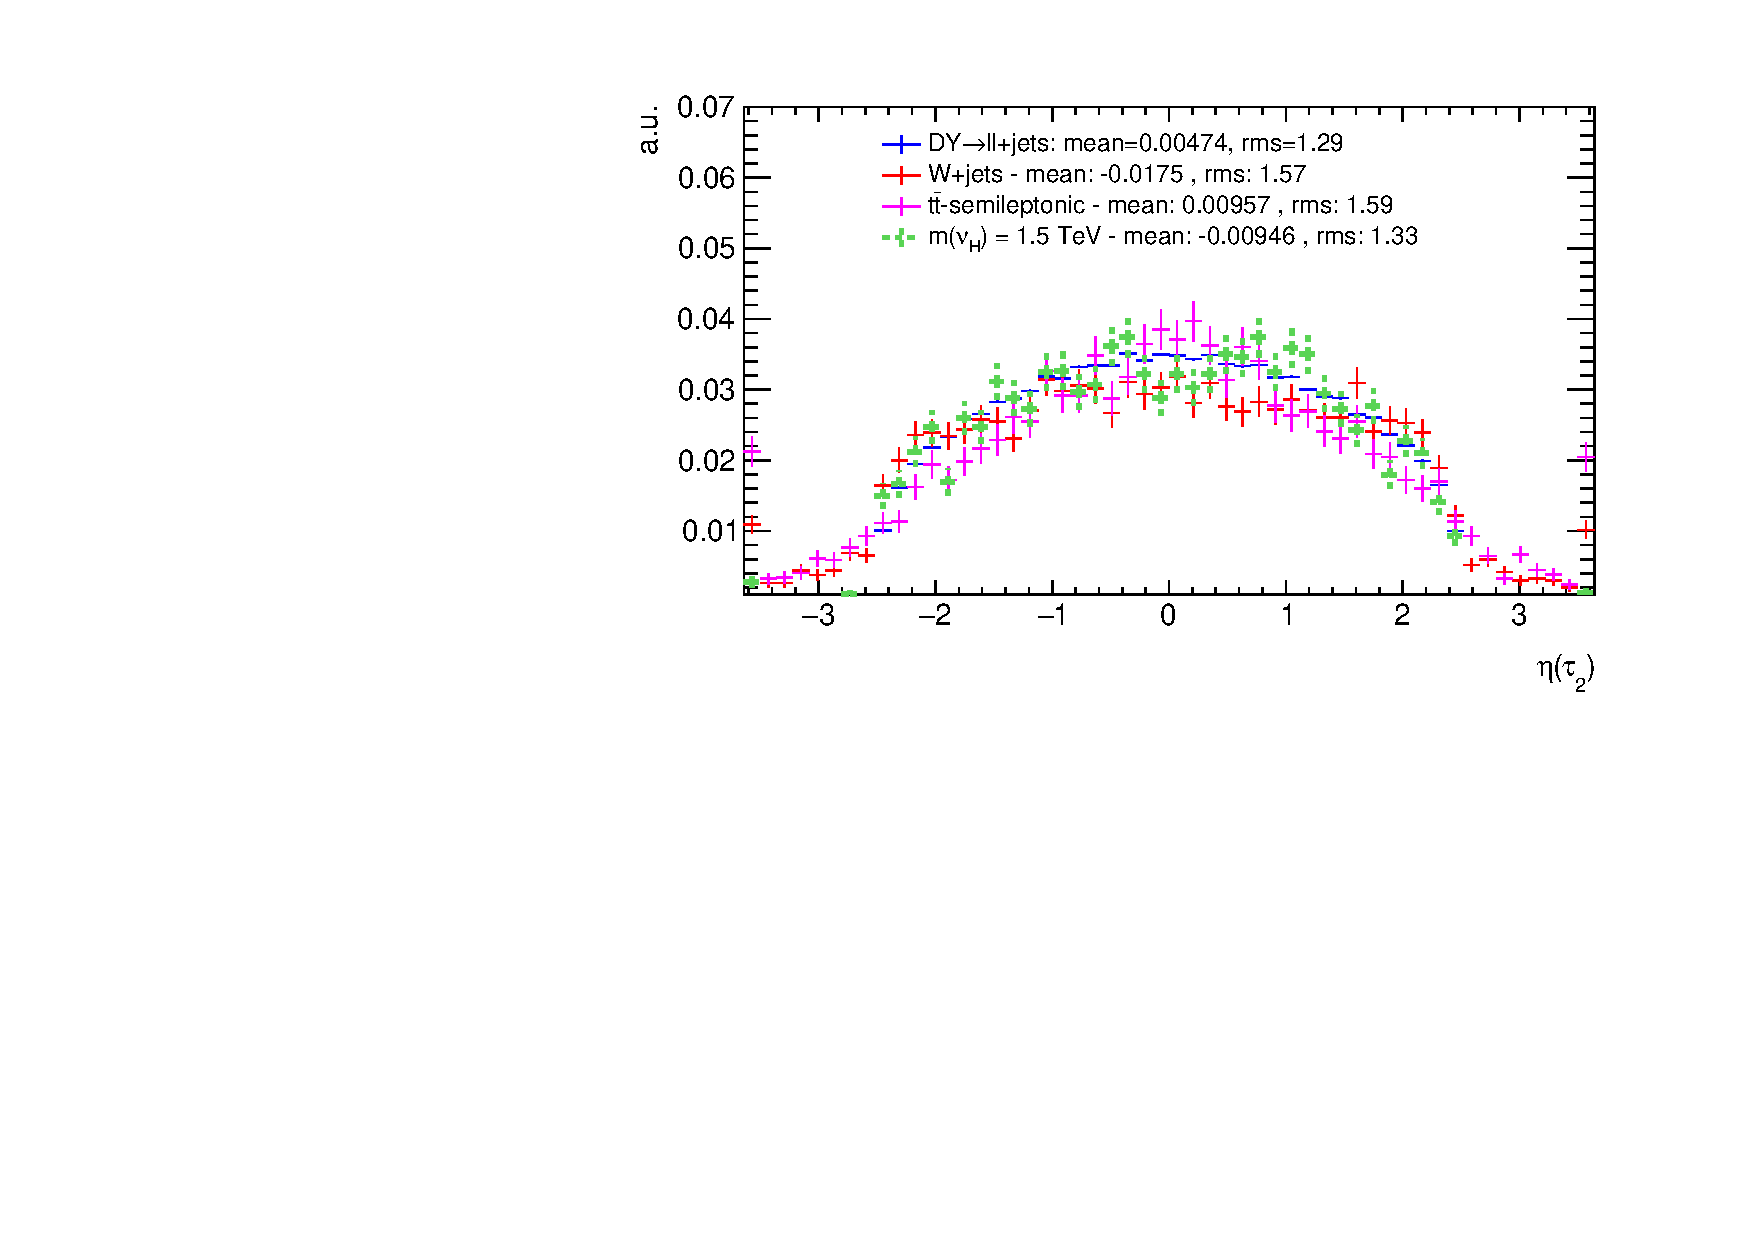
\includegraphics[width=\linewidth]{Plots/tau2_eta_unitNC.pdf}
\caption{Unit plot of $\eta$ from the sub-leading $\tau$ with no cuts}
\label{fig: tau2etaunitNC}
\end{figure}

\begin{figure}
\centering
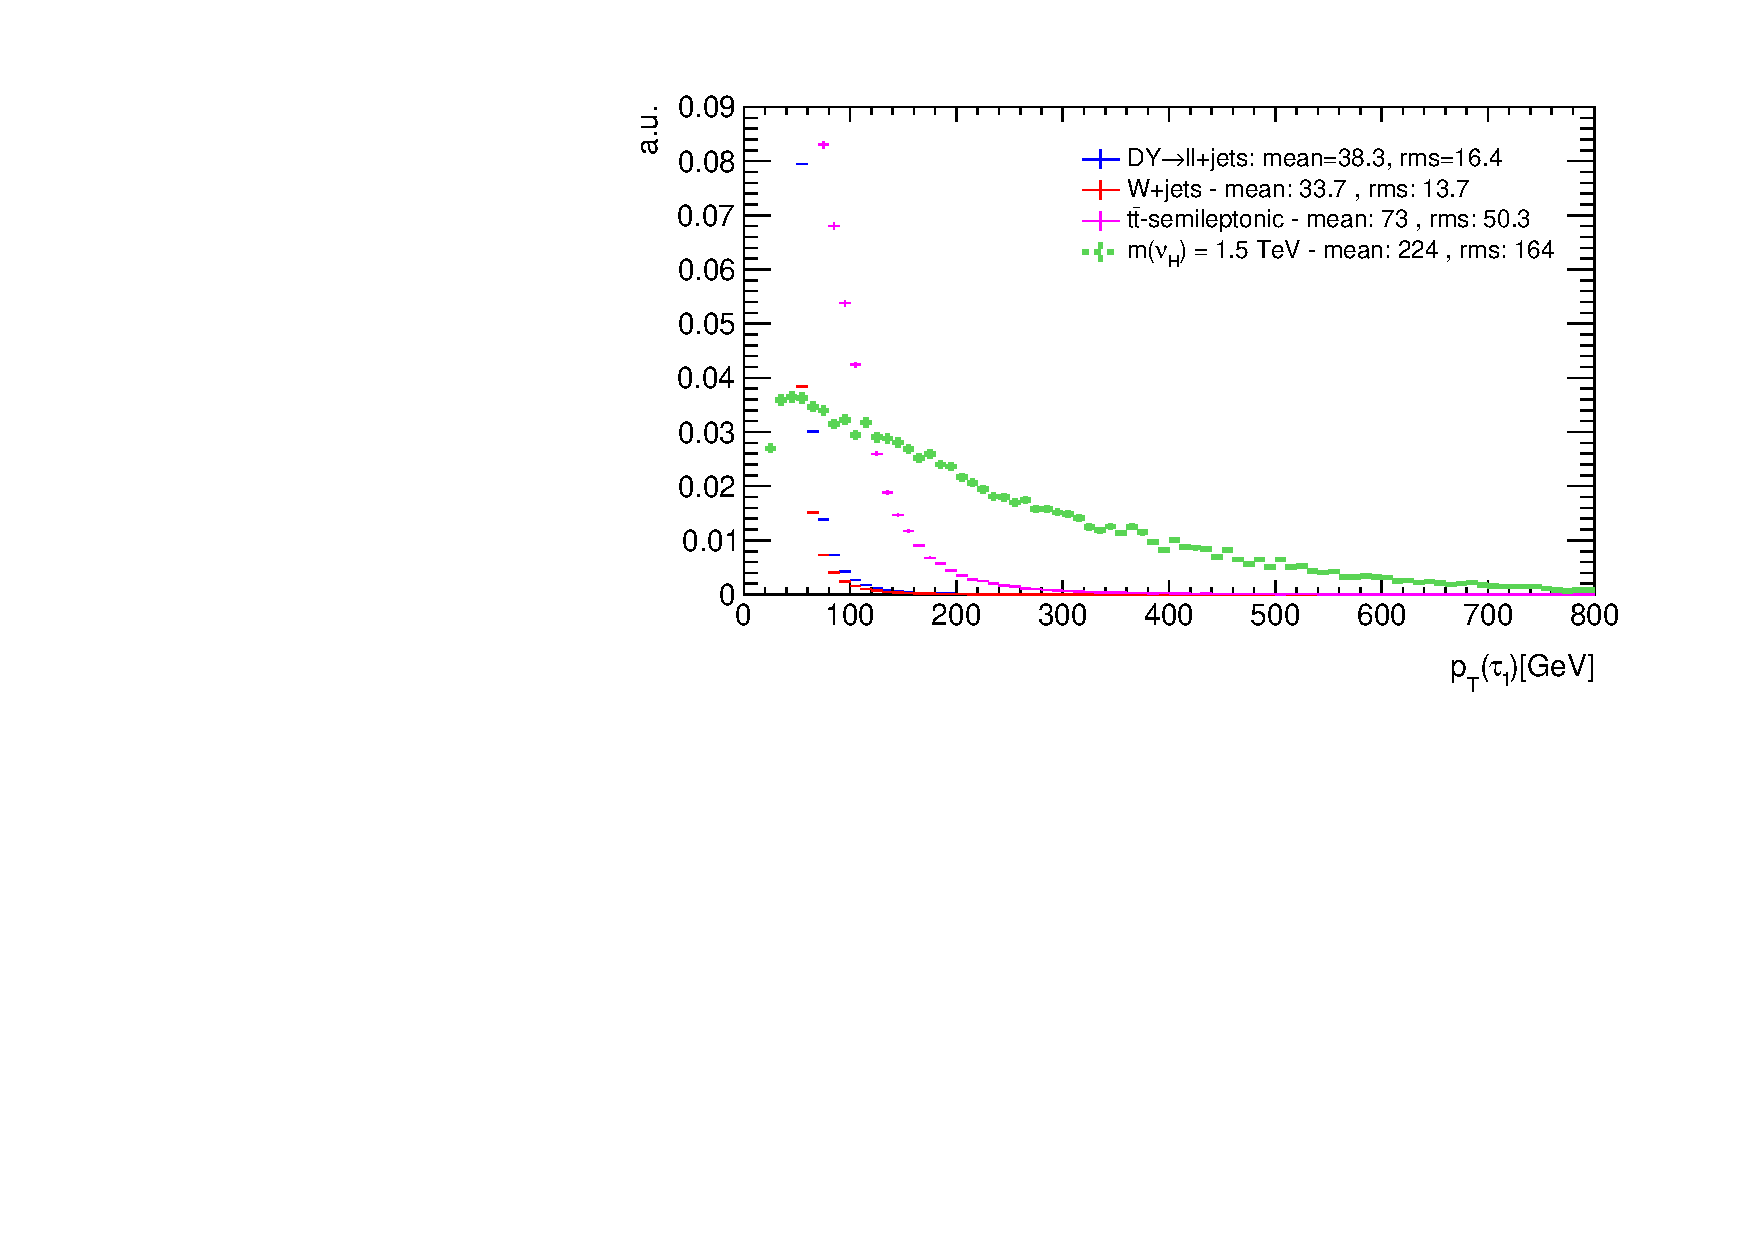
\includegraphics[width=\linewidth]{Plots/tau1_pt_unitNC.pdf}
\caption{Unit plot of $p_{T}$ of leading $\tau$ with no cuts}
\label{fig: tau1ptunitNC}
\end{figure}

To understand the definition of $H_{T}$ and $S_{T}$ mentioned in Chapter \ref{sec:definitions}, the plots in Figure \ref{fig: ptUnitPlots} are shown. The four plots show a separation, in some cases a smaller than others, between the signal and backgrounds distributions. A tendency of the signal jets to have greater transverse momentum than the ones in the backgrounds is shown. This tendency is also displayed for both $\tau$'s. Hence, the distributions of $H_{T}$ and $S_{T}$ should show a similar behaviour because this variables are the result of adding the transverse momentum of jets and $\tau$'s in the event.

\begin{figure}       
        \centering
        \begin{subfigure}[b]{0.475\textwidth}
            \centering
            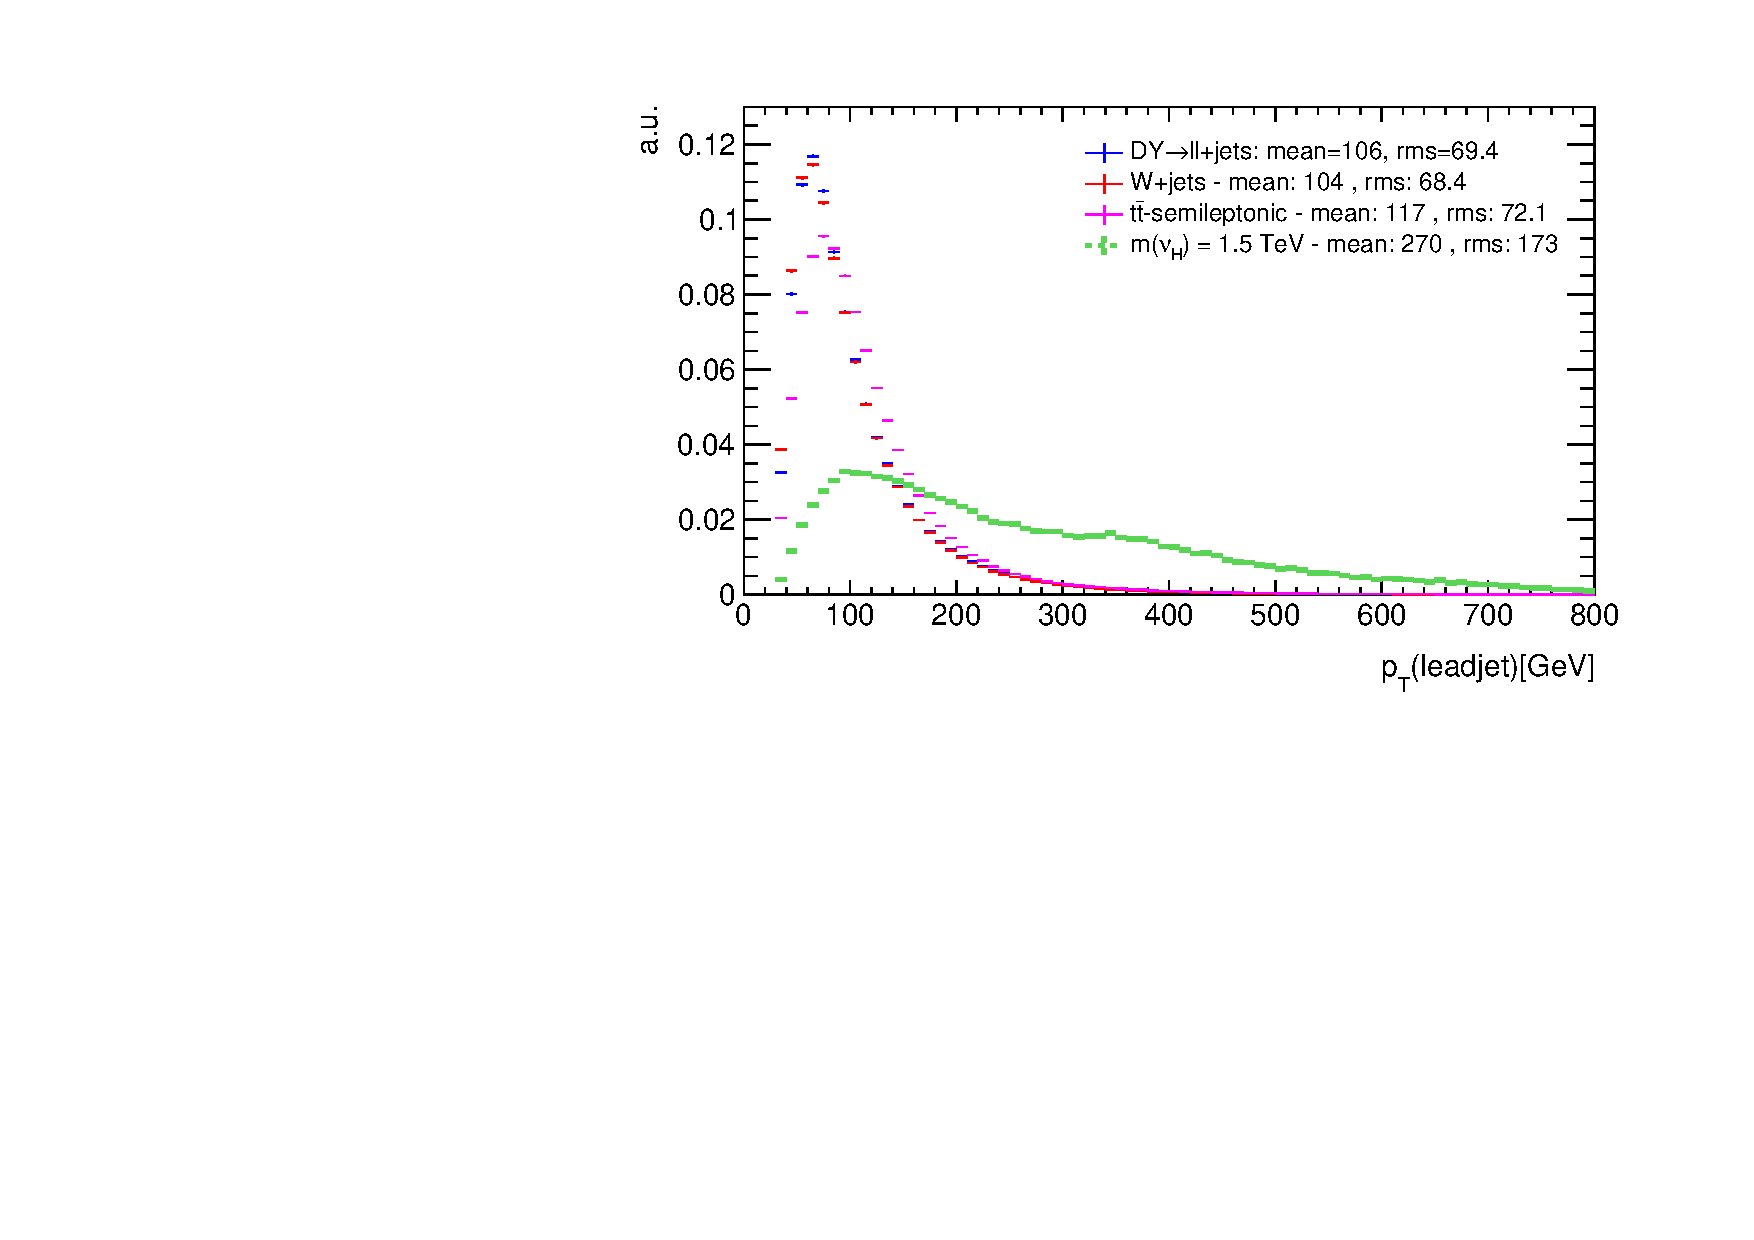
\includegraphics[width=\textwidth]{Plots/ljet_pt_unitNC}
            \caption[]%
            {{\small Leading jet $p_{T}$ unit plot}}    
            %\label{fig:mean and std of net14}
        \end{subfigure}
        \hfill
        \begin{subfigure}[b]{0.475\textwidth}  
            \centering 
            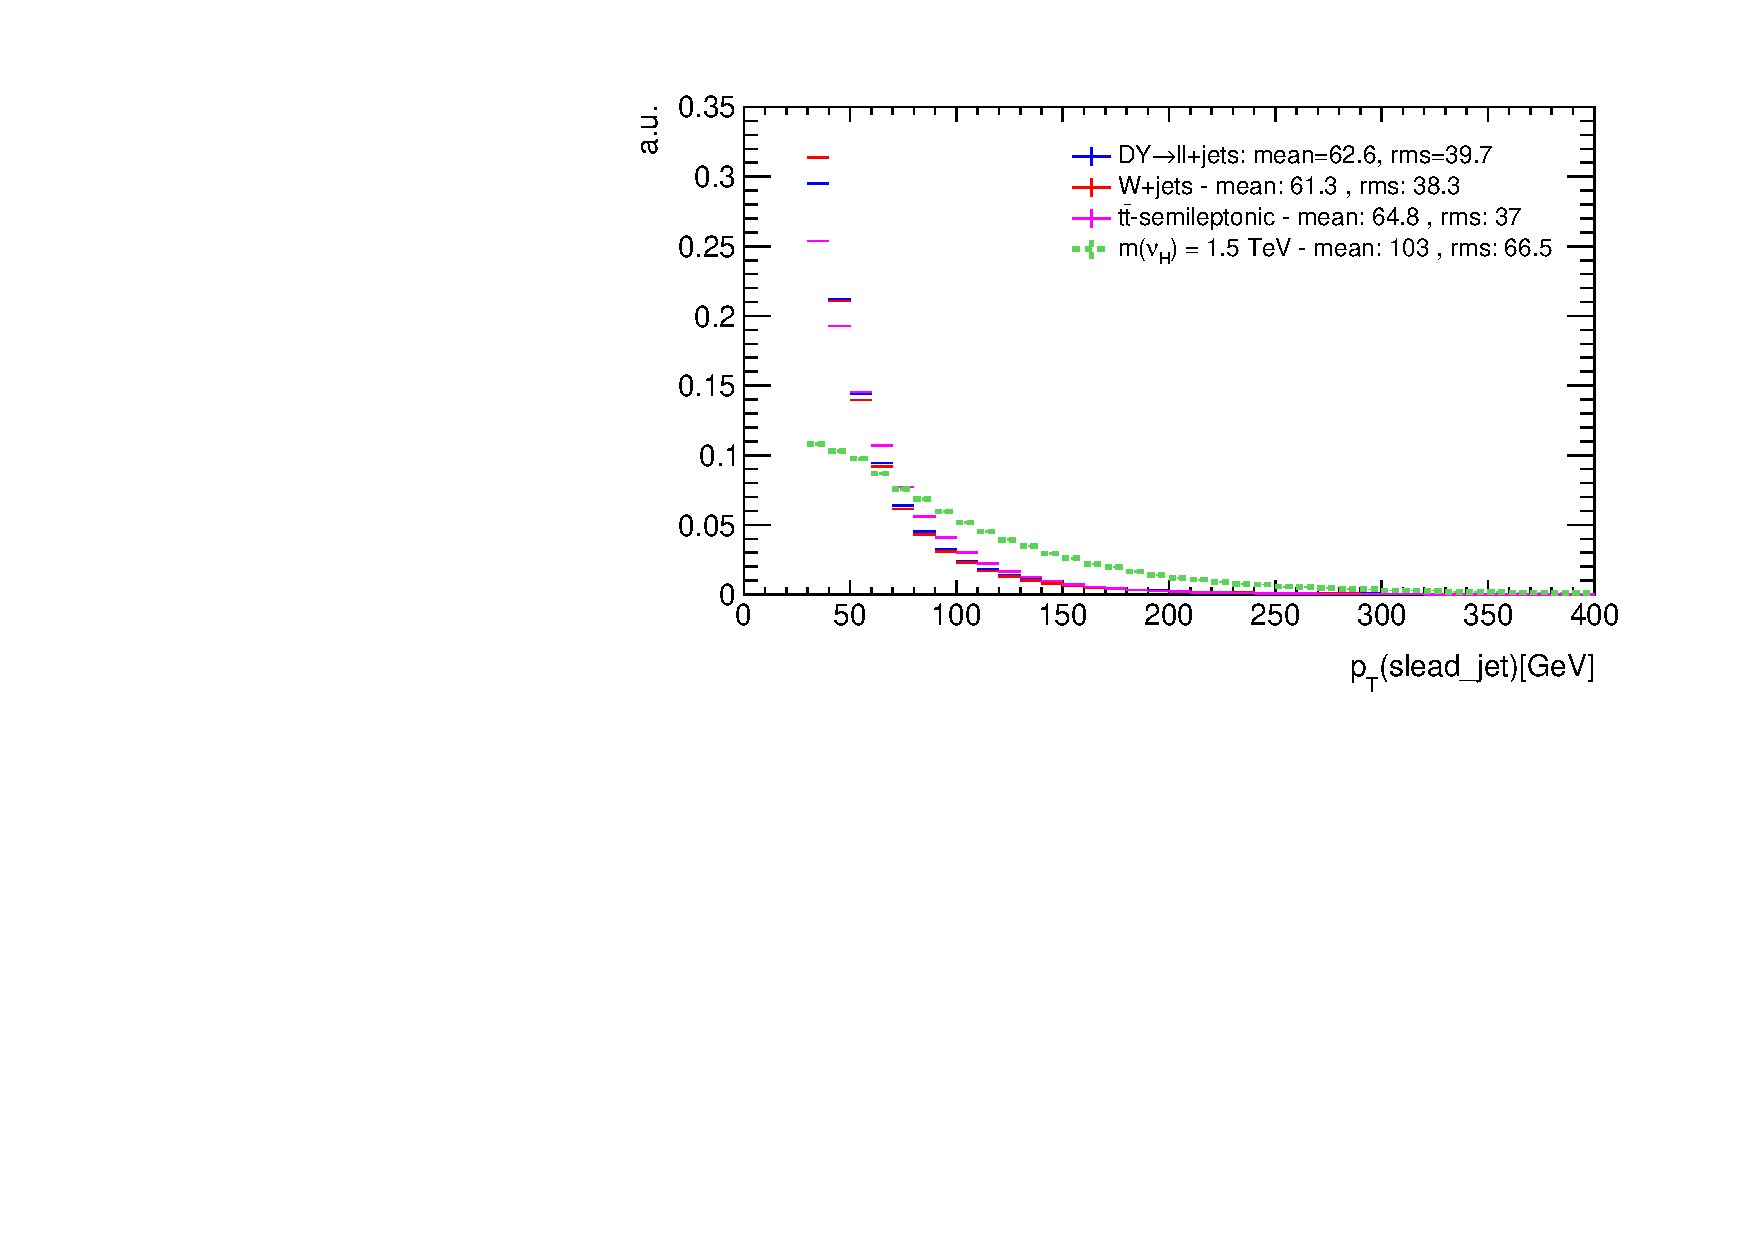
\includegraphics[width=\textwidth]{Plots/sjet_pt_unitNC}
            \caption[]%
            {{\small Sub-leading jet $p_{T}$ unit plot}}    
            %\label{fig:mean and std of net24}
        \end{subfigure}
        \vskip\baselineskip
        \begin{subfigure}[b]{0.475\textwidth}   
            \centering 
            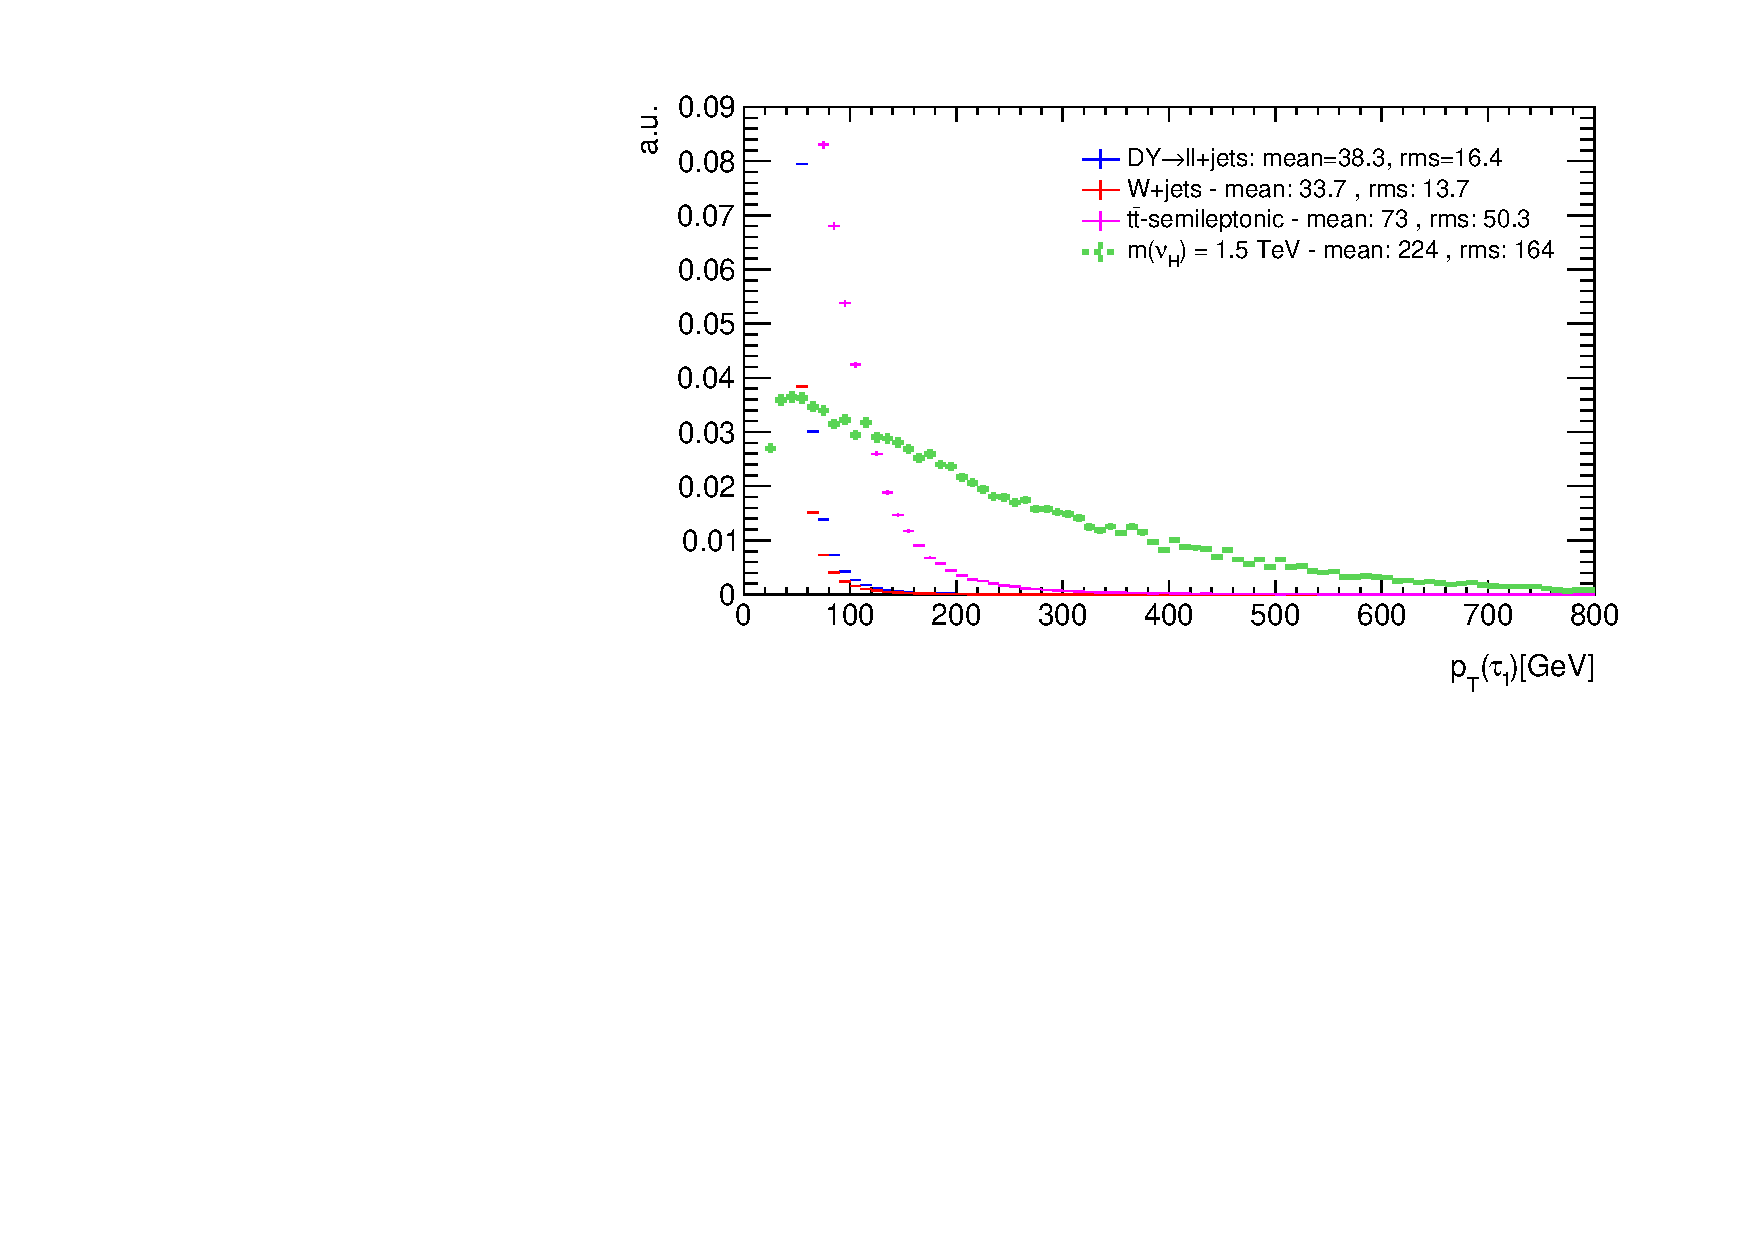
\includegraphics[width=\textwidth]{Plots/tau1_pt_unitNC}
            \caption[]%
            {{\small Leading $\tau$ $p_{T}$ unit plot}}    
            %\label{fig:mean and std of net34}
        \end{subfigure}
        \quad
        \begin{subfigure}[b]{0.475\textwidth}   
            \centering 
            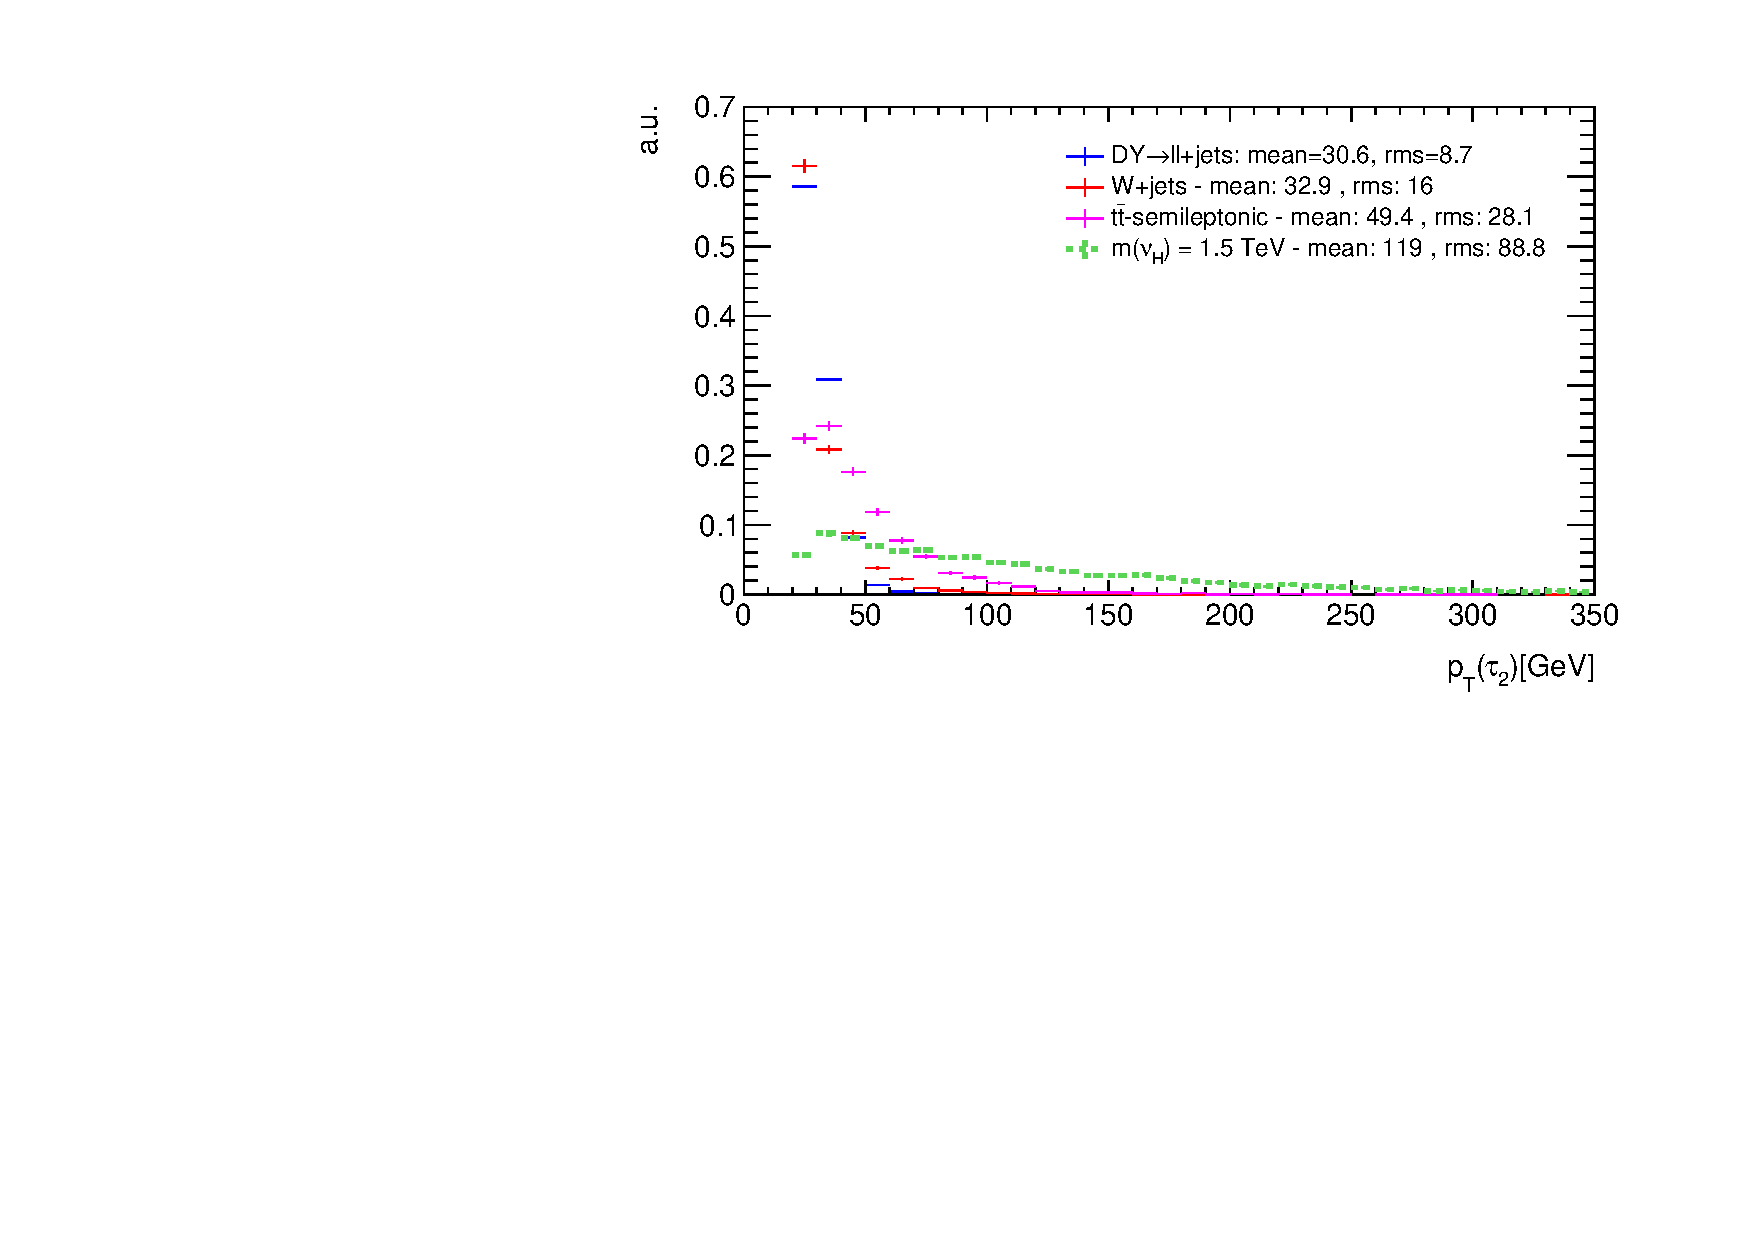
\includegraphics[width=\textwidth]{Plots/tau2_pt_unitNC}
            \caption[]%
            {{\small Sub-leading $\tau$ $p_{T}$ unit plot}}    
            %\label{fig:mean and std of net44}
        \end{subfigure}
        \caption[ $p_T$ unit plots for different bodies in the event]
        {\small $p_T$ unit plots for different bodies in the event} 
         \label{fig: ptUnitPlots}
\end{figure}

In Figures \ref{fig: HTunitNC} and \ref{fig: STunitNC}, the normalized plots with no cuts of $H_{T}$ and $S_{T}$ are shown. It can be seen that indeed a greater separation between signal and background was achieved. Unlike the distributions of the $\tau$'s and jets transverse momentum, the maxima of $H_{T}$ and $S_{T}$ lie outside the backgrounds distributions. Furthermore, the background that overlaps at a greater energy with the signal corresponds to $t\bar{t}$. Taking into account what was mentioned in Section \ref{sec: selectionCriteria}, the overlap between the signal and this background could be reduced with the cut related with the number of B-jets in the event. This is why this two variables need to be studied closer in the analysis.

\begin{figure}
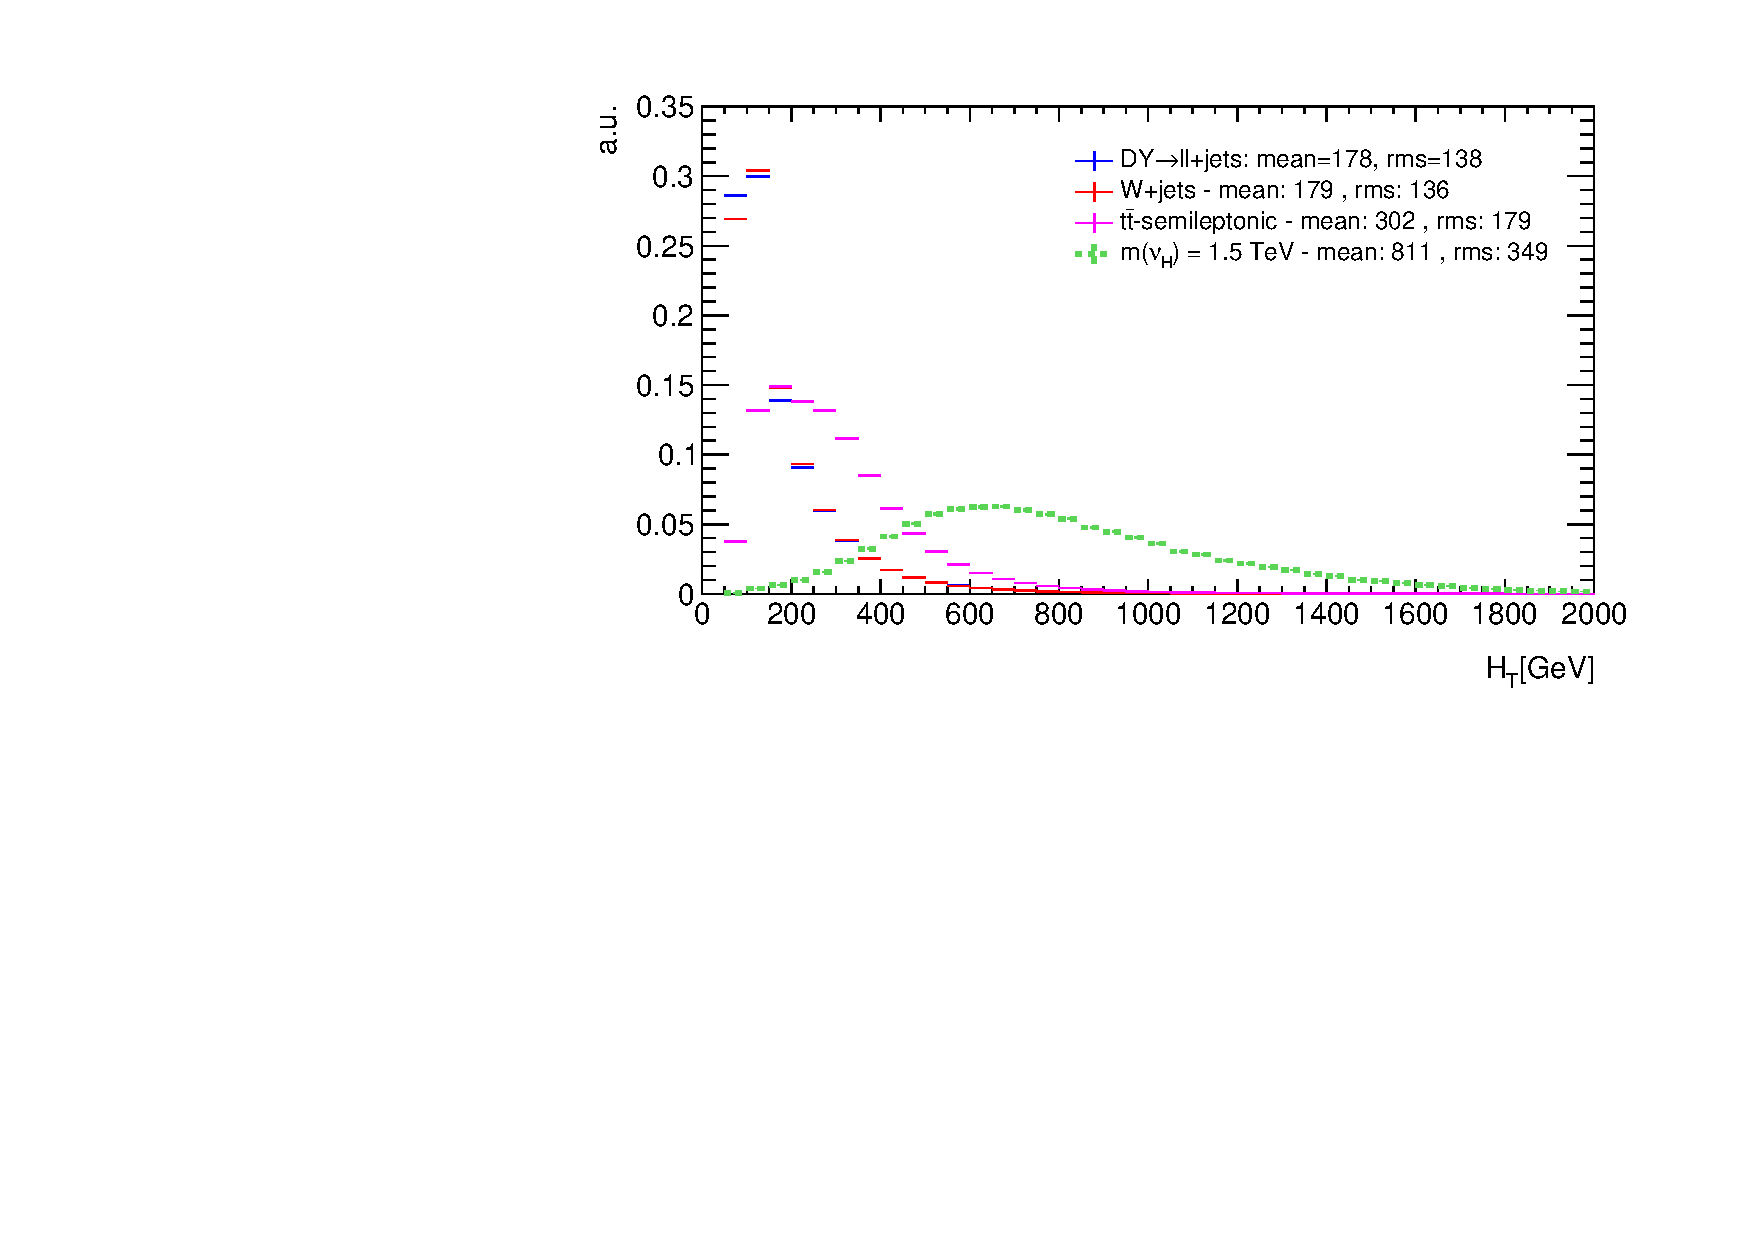
\includegraphics[width=\linewidth]{Plots/HT_unitNC.pdf}
\caption{Unit plot of $H_{T}$ with no cuts}
\label{fig: HTunitNC}
\end{figure}

\begin{figure}
\centering
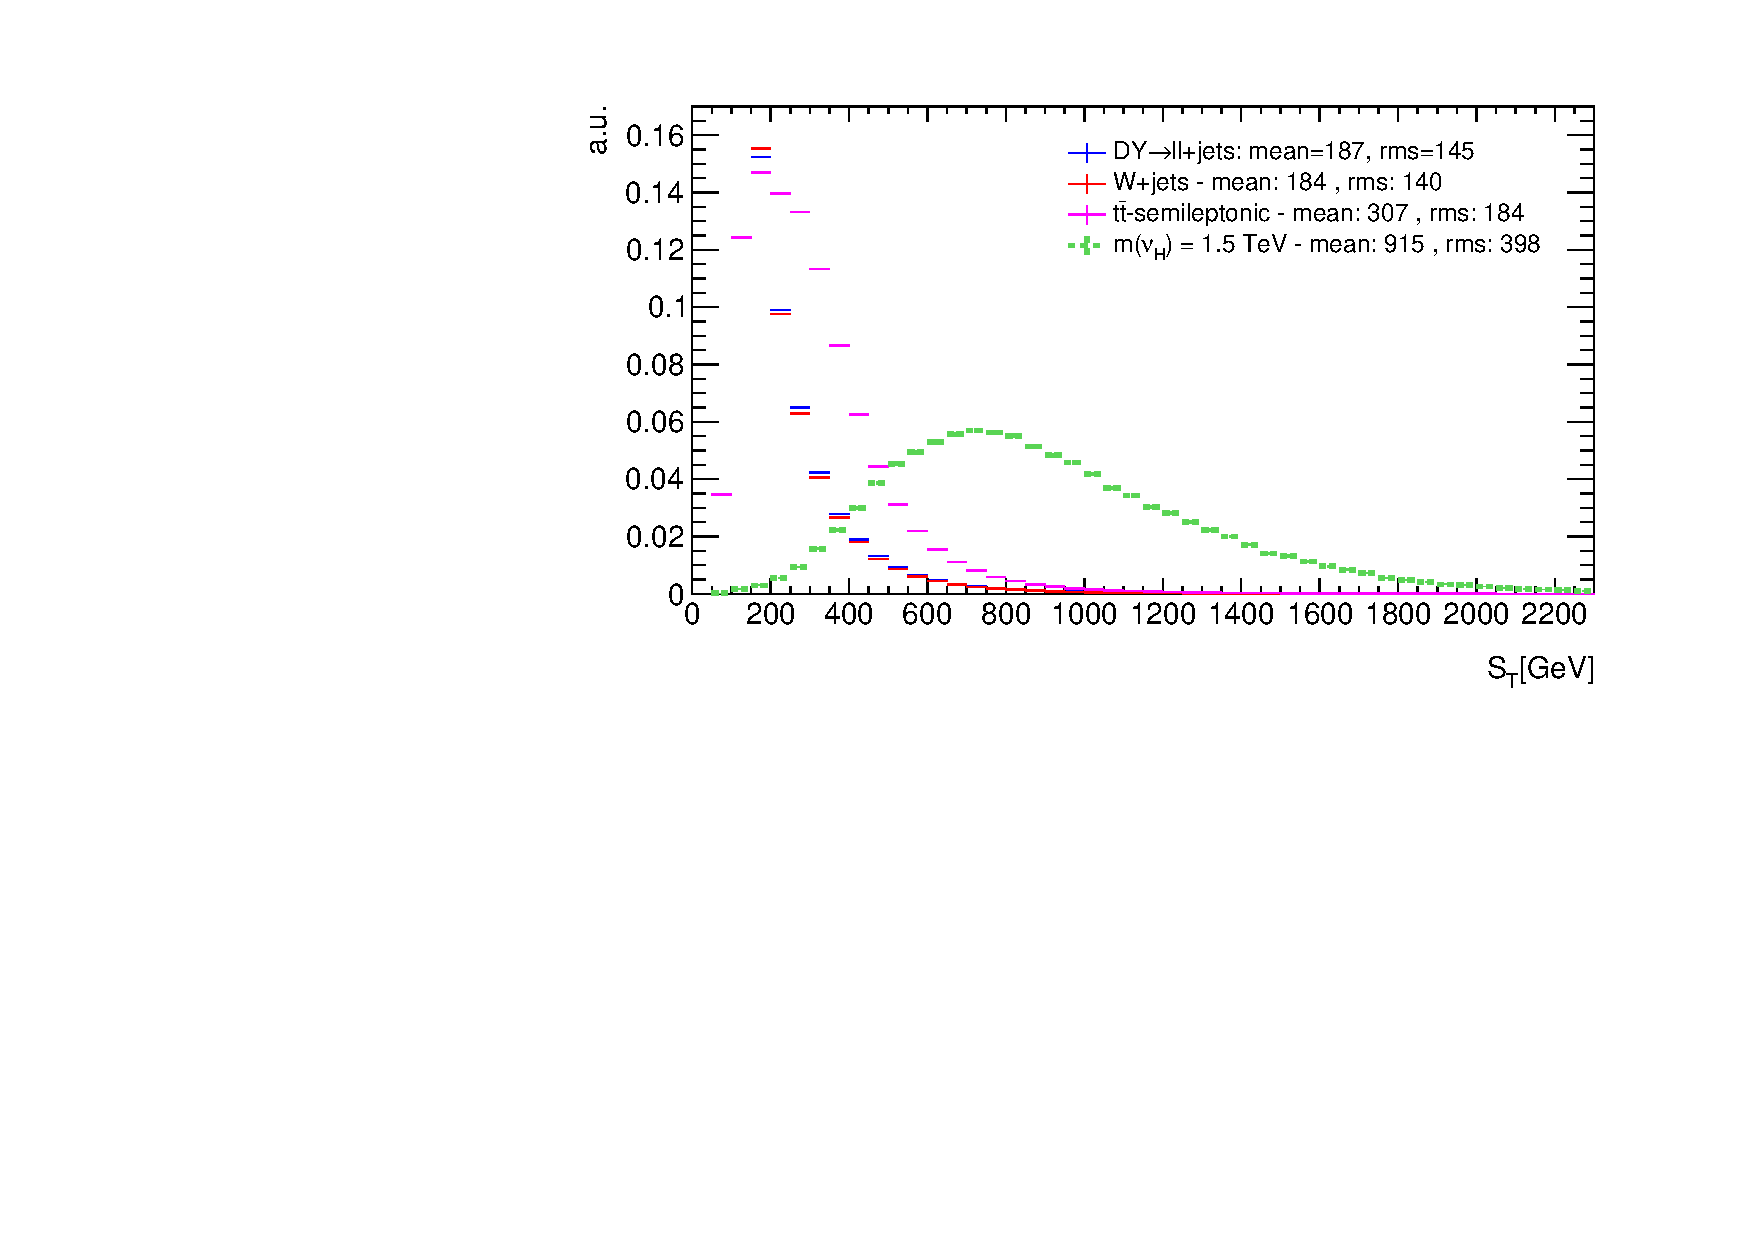
\includegraphics[width=\linewidth]{Plots/ST_unitNC.pdf}
\caption{Unit plot of $S_{T}$ with no cuts}
\label{fig: STunitNC}
\end{figure}

Another variable relevant for the analysis was found out to be $m(jj)$. The reason for a further analysis of this variable is shown in Figure \ref{fig: mjjUnitNC}. As in the case of $H_{T}$ and $S_{T}$, the distribution of the mass of the Di-Jet Pair shows a separation between the signal and the three backgrounds. Furthermore, it shows a greater separation than the one observed for both $H_{T}$ and $S_{T}$. That is why, the variable $m(jj)$, or the total mass of the Di-Jet Pair, has to be studied more closely, because it shows potential for a separation between signal and backgrounds.

\begin{figure}
\centering
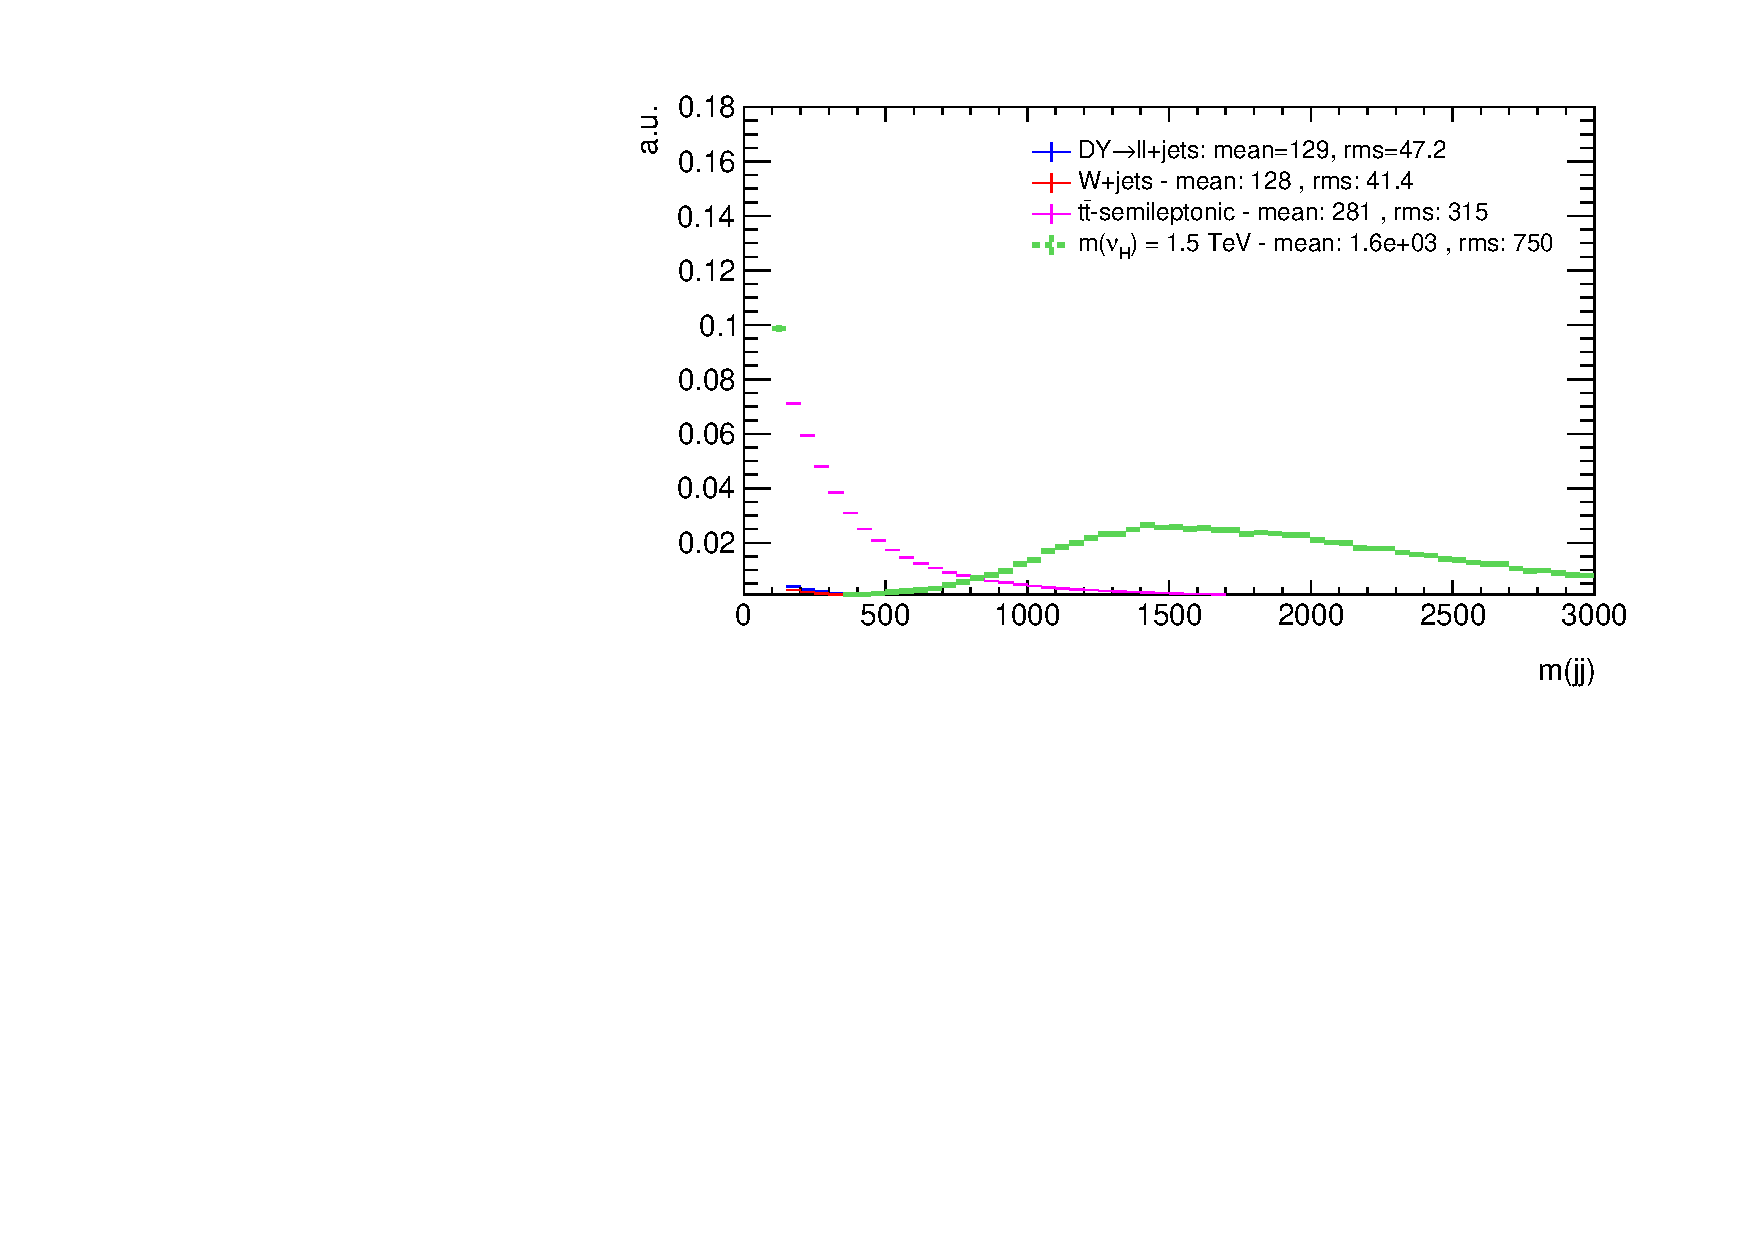
\includegraphics[width=\linewidth]{Plots/mjj_unitNC.pdf}
\caption{Unit plot of $m(jj)$ with no cuts}
\label{fig: mjjUnitNC}
\end{figure}


\section{Stack Plots}\label{section: stackPlots}

The plots shown in this section are the ones corresponding with the relevant variables mentioned in section \ref{sec: Normalized Distributions}. All the plots presented are normalized to the cross section of each process and to a luminosity of 50 $\text{fb}^{-1}$. Also, since the amount of signal events is small after applying all the selection criteria, the number of events axis is in a logarithmic scale. This allows to examine the distribution shape more easily when the number of events of a distribution is small. 

In Figures \ref{fig: HT2tausMet50} and \ref{fig: HT2tausMet60}, the stack plots for the $H_{T}$ distributions, with $\slashed{E}_{T}$ cuts of 50 and 60 GeV respectively, are shown. Comparing these two plots, it is observed that an increase of 10 GeV of the cut in the transverse missing energy is useful to separate the signal from the backgrounds. Focusing in the amount of background shown in Figures \ref{fig: HT2tausMet50} and \ref{fig: HT2tausMet60}, it can be seen that with the increase in the $\slashed{E}_{T}$ cut, the amount of background events was reduced from approximately 160 to about 40. Besides, with the new missing tranvserse energy cut, the amount of signal events was not significantly reduced. A similar conclusion can be drawn from Figures \ref{fig: ST2tausMet50} through \ref{fig: mjj2tauMet60}. The reduction in background resulting from this cut increase is mainly due to the fact of almost completely eliminating the W+jets background. Comparing the amount of W+jets in Figures \ref{fig: HT2tausMet50}, \ref{fig: ST2tausMet50}, and \ref{fig: mjj2tausMet50} with the amount present in Figures \ref{fig: HT2tausMet60} and \ref{fig: ST2tausMet60}, and \ref{fig: mjj2tauMet60}, it can be clearly seen that the background coming from W+jets is eliminated. It could be argued that a stronger cut in the missing transverse energy would increase the separation between signal and background. However, analyzing the $\slashed{E}_{T}$ distribution in \ref{fig: MET1tauMet60}, it can be seen that a further increase in the cut would also eliminate a considerable amount of signal events. The reasons presented in this paragraphs are why the increase of 10 GeV in the $\slashed{E}_{T}$ cut is convenient for separating signal from backgrounds.

As expected from the analysis performed in Section \ref{sec: Normalized Distributions}, the variables $H_{T}$ and $S_{T}$ show separation between signal and backgrounds. The latter can be observed in Figures \ref{fig: HT2tausMet50} and \ref{fig: HT2tausMet60} for $H_{T}$, and Figures \ref{fig: ST2tausMet50} and \ref{fig: ST2tausMet60} for $S_{T}$. However, from these four plots it can also be concluded that $S_{T}$ is a better variable than $H_{T}$ for this study. This conclusion can be drawn from the fact that the signal distribution decays slower in the $S_{T}$ variable than in $H_{T}$. These four plots required two taus in the event. The leading tau had a requirement of minimum transverse momentum of 50 GeV and the subleading tau a minimum $p_{T}$ of 20 GeV.


Although both $H_{T}$ and $S_{T}$ allow to obtain a separation between signal and backgrounds, the Di-Jet mass, or $m(jj)$, has a distribution that would allow to distinguish better signal and backgrounds. This fact is shown in Figures \ref{fig: mjj2tausMet50} and \ref{fig: mjj2tauMet60}, where the signal decays slower than in the cases of $H_{T}$ and $S_{T}$ for values where the backgrounds are not longer present. This flatter distribution compared to $H_{T}$ and $S_{T}$ allows to have a greater number of events outside the regions where the backgrounds are present for the Di-Jet mass variable. It has to be mentioned that these two plots are also for the case where two taus, with the conditions mentioned in the previous paragraph, were required in the event. 

A variable that in the normalized plot analysis did not show separation between the signal and the background was the transverse mass between the tau and the missing transverse energy. However, looking for other potentially useful varibles for the analysis, the stack plot $m_{T}(\tau, \slashed{E}_{T})$ showed good separation between signal and backgrounds. This stack plot is presented in Figure \ref{fig: mT2tausMet60}, and it can be seen that the signal separates from the background distributions from a value of 300 GeV. However, for the case requiring two taus in the event, the Di-Jet mass would be more useful, because it decays slower than the $m_{T}$ distribution. 

In Figures \ref{fig: HT2tausMet60}, \ref{fig: ST2tausMet60}, \ref{fig: mjj2tauMet60}, and \ref{fig: mT2tausMet60}, the distributions for the six heavy neutrinos mass values that were considered in the analysis are shown. Taking into account the discussion presented in Chapter \ref{chapter: neutrinoSearches}, the processes of heavy neutrino production with smaller heavy neutrino mass values have larger cross sections. That is why it would be expected that the distributions mentioned at the beginning of this paragraph should have a larger number of events than the ones that correspond to larger heavy neutrino mass values. However, the signal distributions shown in Figures \ref{fig: HT2tausMet60}, \ref{fig: ST2tausMet60}, \ref{fig: mjj2tauMet60}, and \ref{fig: mT2tausMet60} do not display this behaviour, because in none of this distributions shown the signal with 0.1 TeV mass value has the largest number of events. This reduction in the number of events for processes with larger cross section is caused by the selection criteria implemented for the analysis. Most of the particles in the final state of the process come from the decay of the heavy neutrino, so if the smaller the mass of the heavy neutrino, the smaller the energy of the particles resulting from the neutrino decay. Since many of the selection criteria established for this analysis are related with the energy of the particle, the number of events that pass the selection criteria decreases when the mass of the heavy neutrino decreases. This is why the signal values that have bigger cross sections do not have greater number of events than the ones that have smaller cross sections. Nevertheless, for mass values bigger than 1.0 TeV, the distributions do follow the rule of having more number of events if the cross section is larger. 

\begin{figure}[H]
\centering
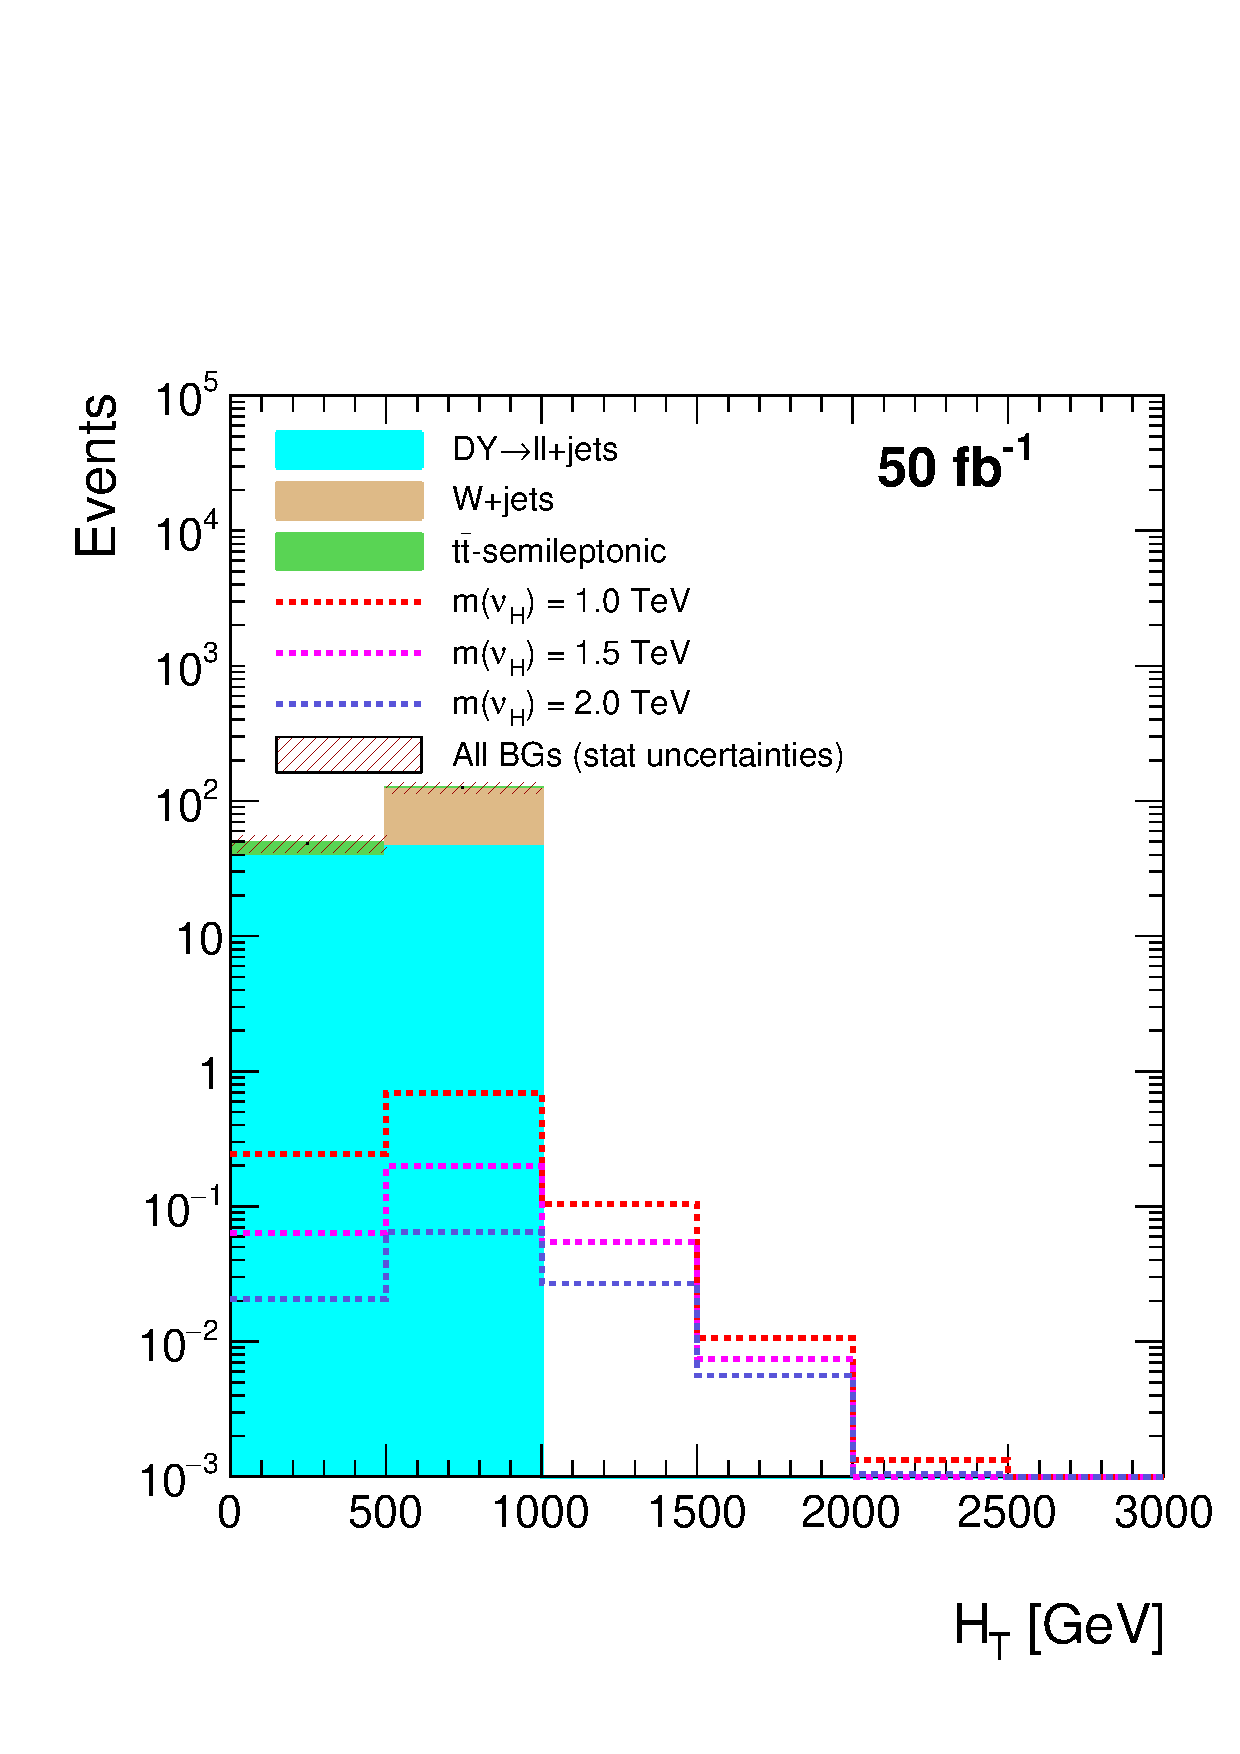
\includegraphics[width=\linewidth]{StackPlots/HT_2taus_met50_50ifb.pdf}
\caption{Stack plot of $H_{T}$ requiring two taus in the event and with $\slashed{E}_{T} > 50$}
\label{fig: HT2tausMet50}
\end{figure}

\begin{figure}[H]
\centering
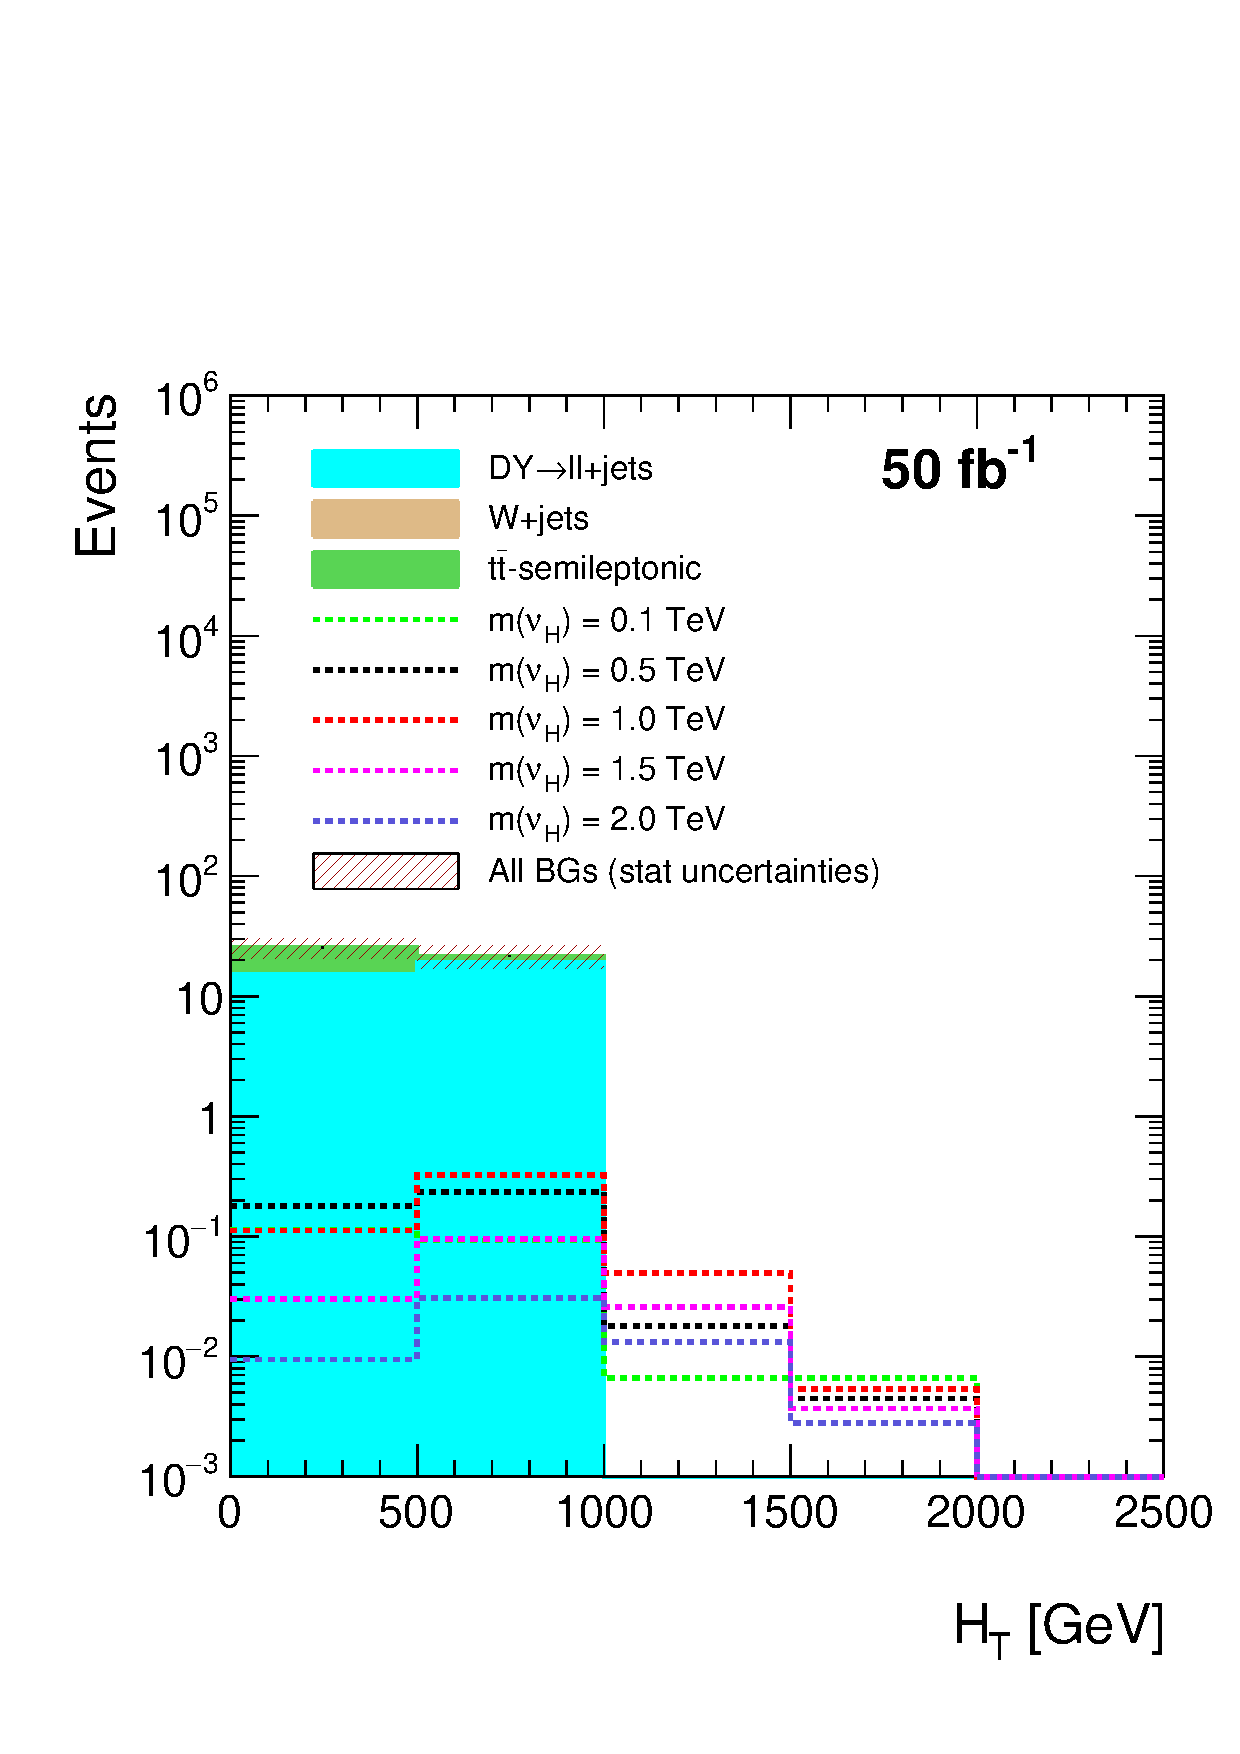
\includegraphics[width=\linewidth]{StackPlots/HT_2Taus_met60_50ifb_2moreSignals.pdf}
\caption{Stack plot of $H_{T}$ requiring two taus in the event and with $\slashed{E}_{T} > 60$}
\label{fig: HT2tausMet60}
\end{figure}



\begin{figure}[H]
\centering
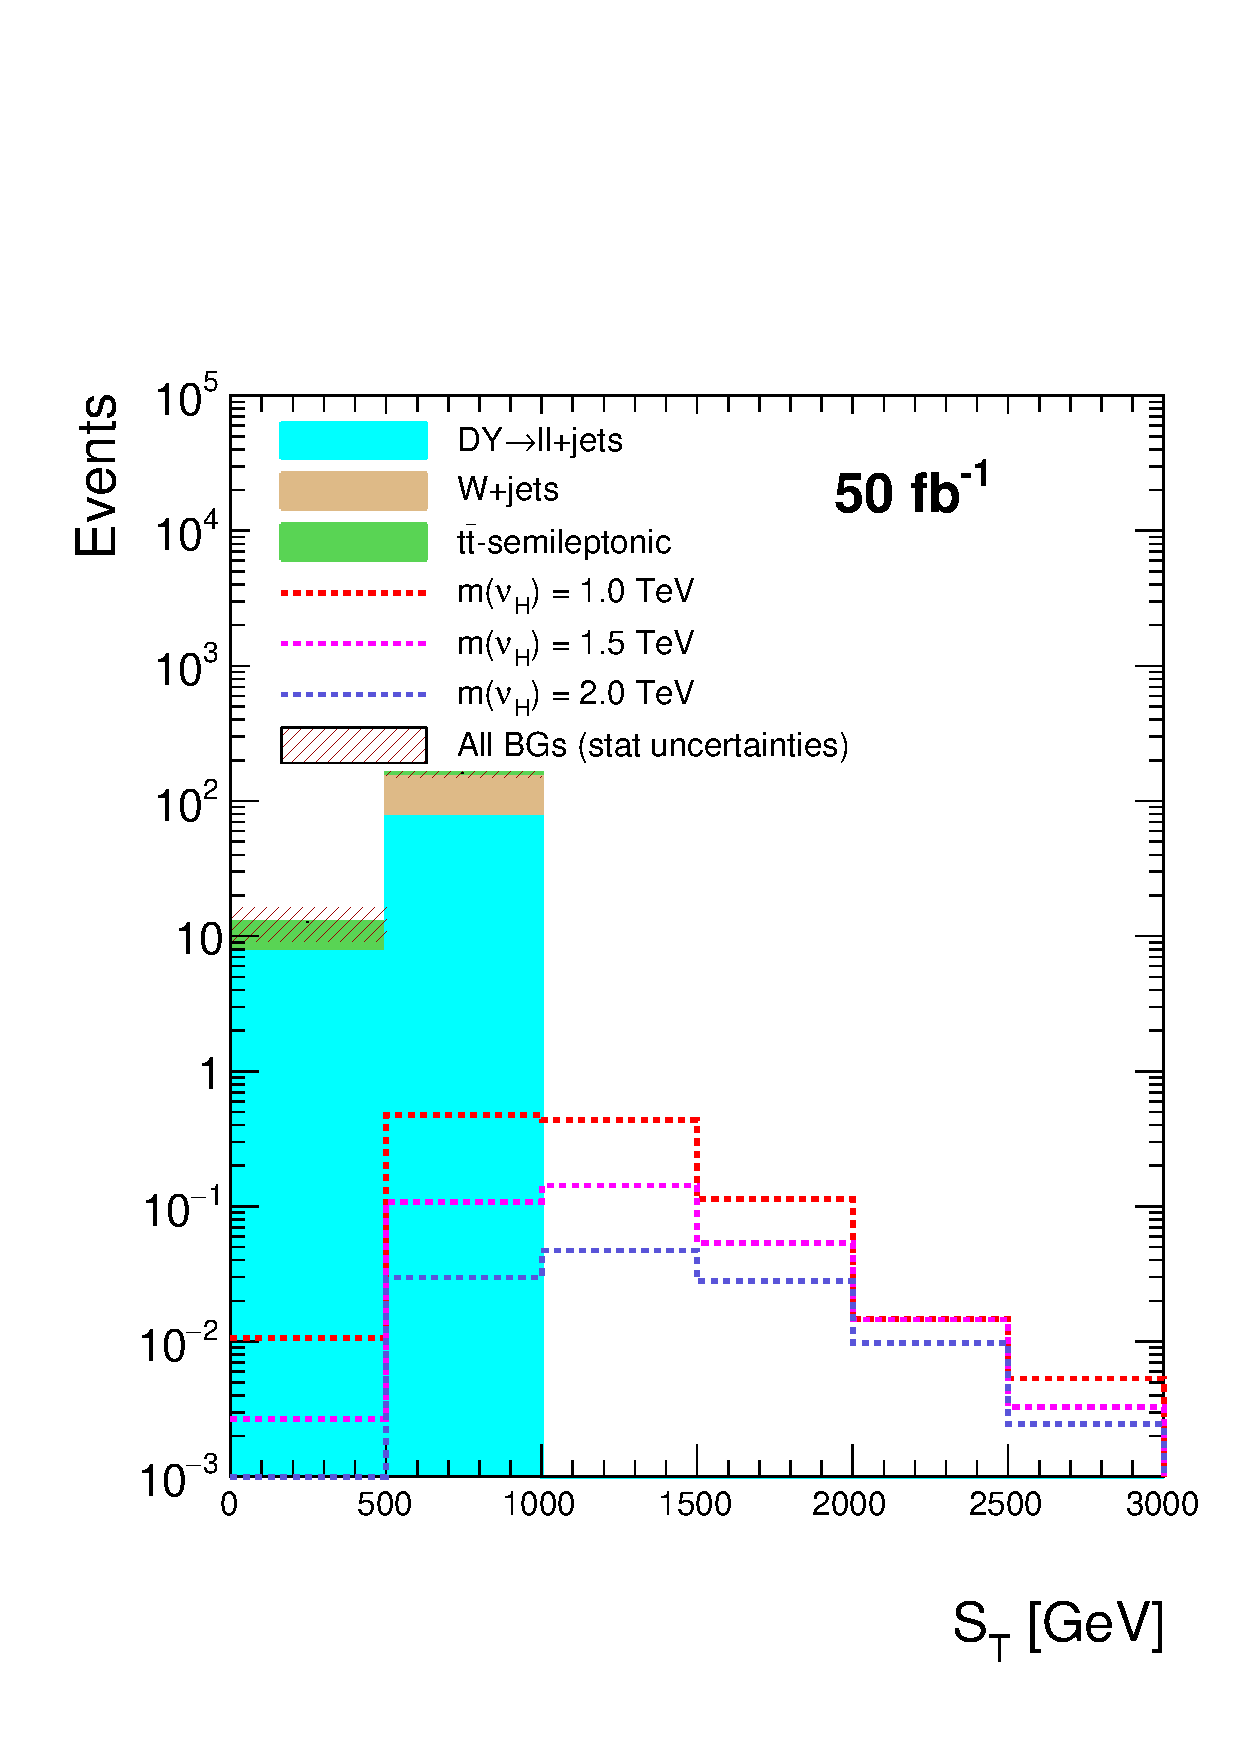
\includegraphics[width=\linewidth]{StackPlots/ST_2taus_met50_50ifb.pdf}
\caption{Stack plot of $S_{T}$ requiring two taus in the event and with $\slashed{E}_{T} > 50$}
\label{fig: ST2tausMet50}
\end{figure}


\begin{figure}[H]
\centering
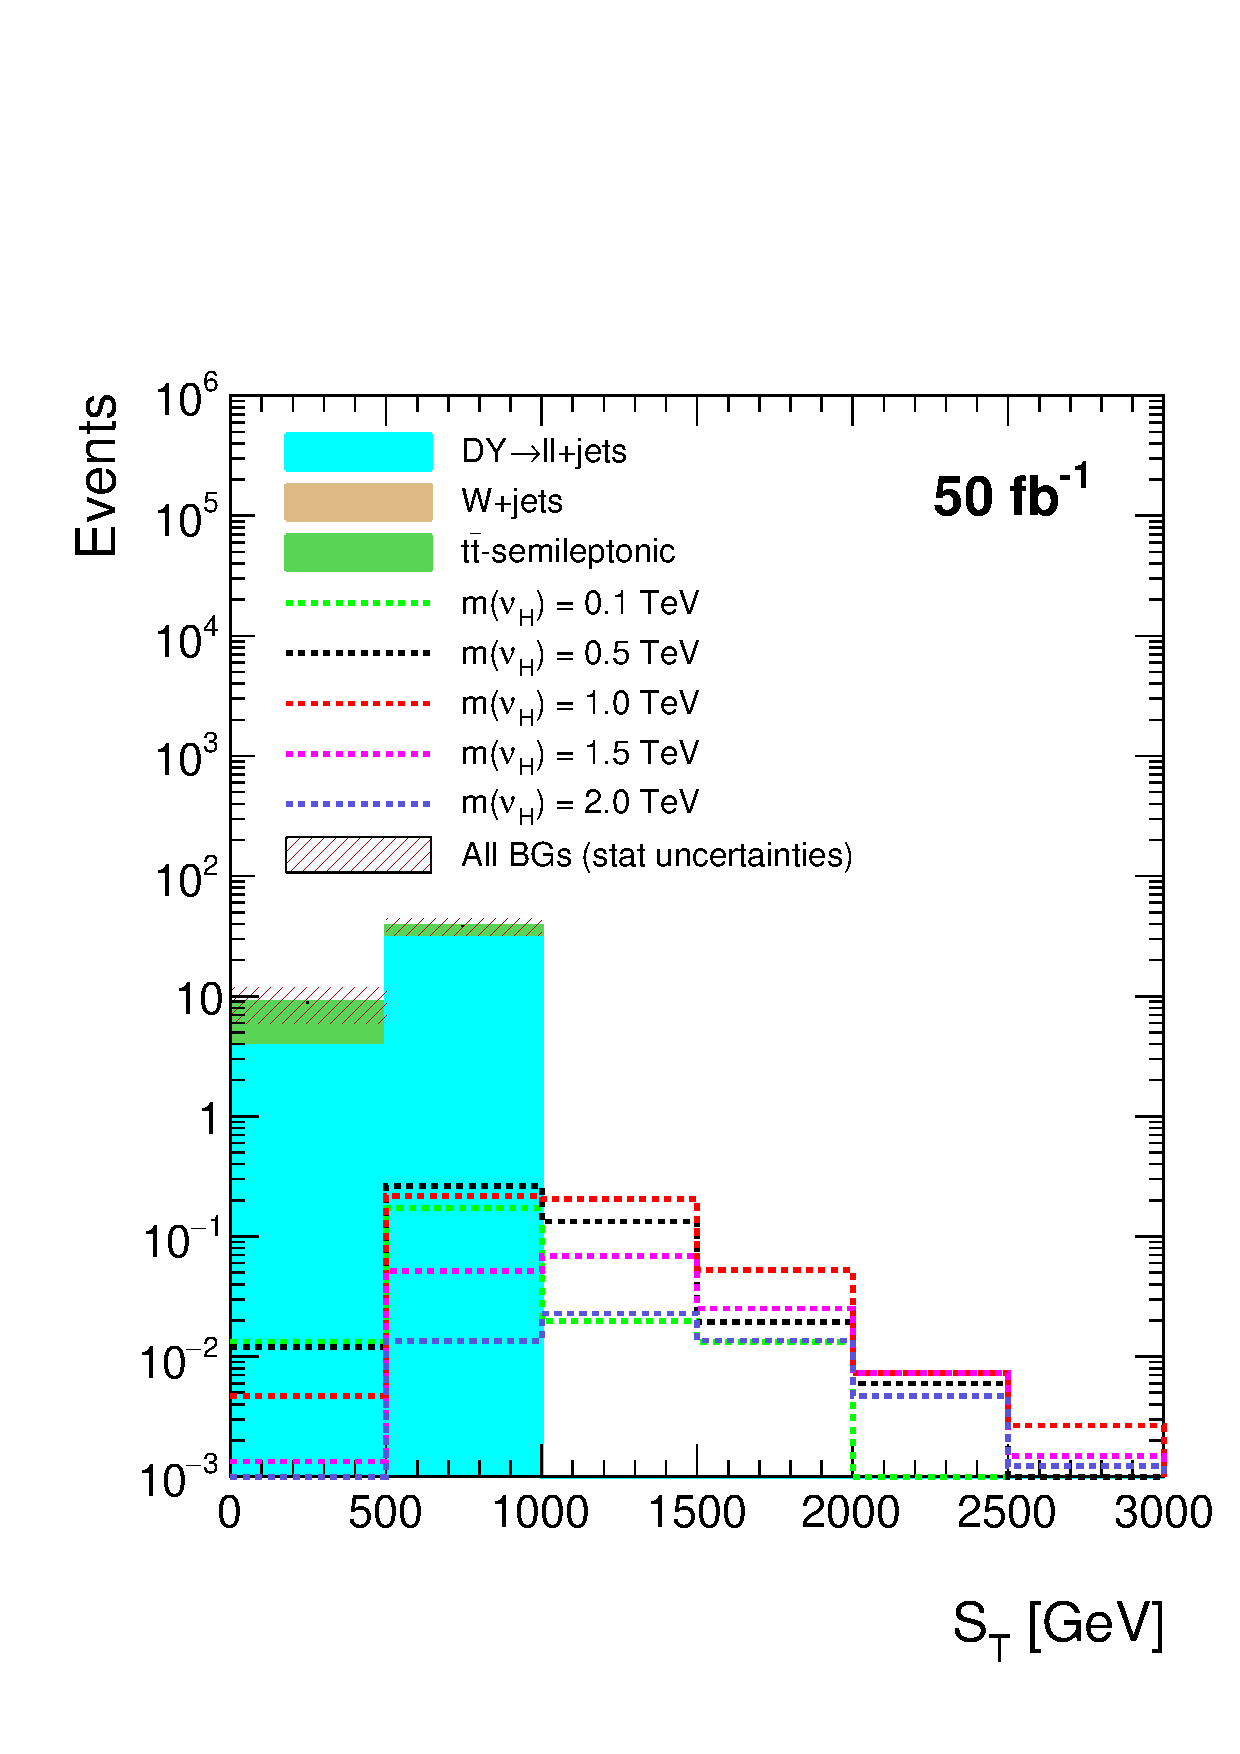
\includegraphics[width=\linewidth]{StackPlots/ST_2Taus_met60_50ifb_2moreSignals.pdf}
\caption{Stack plot of $S_{T}$ requiring two taus in the event and with $\slashed{E}_{T} > 60$}
\label{fig: ST2tausMet60}
\end{figure}



\begin{figure}[H]
\centering
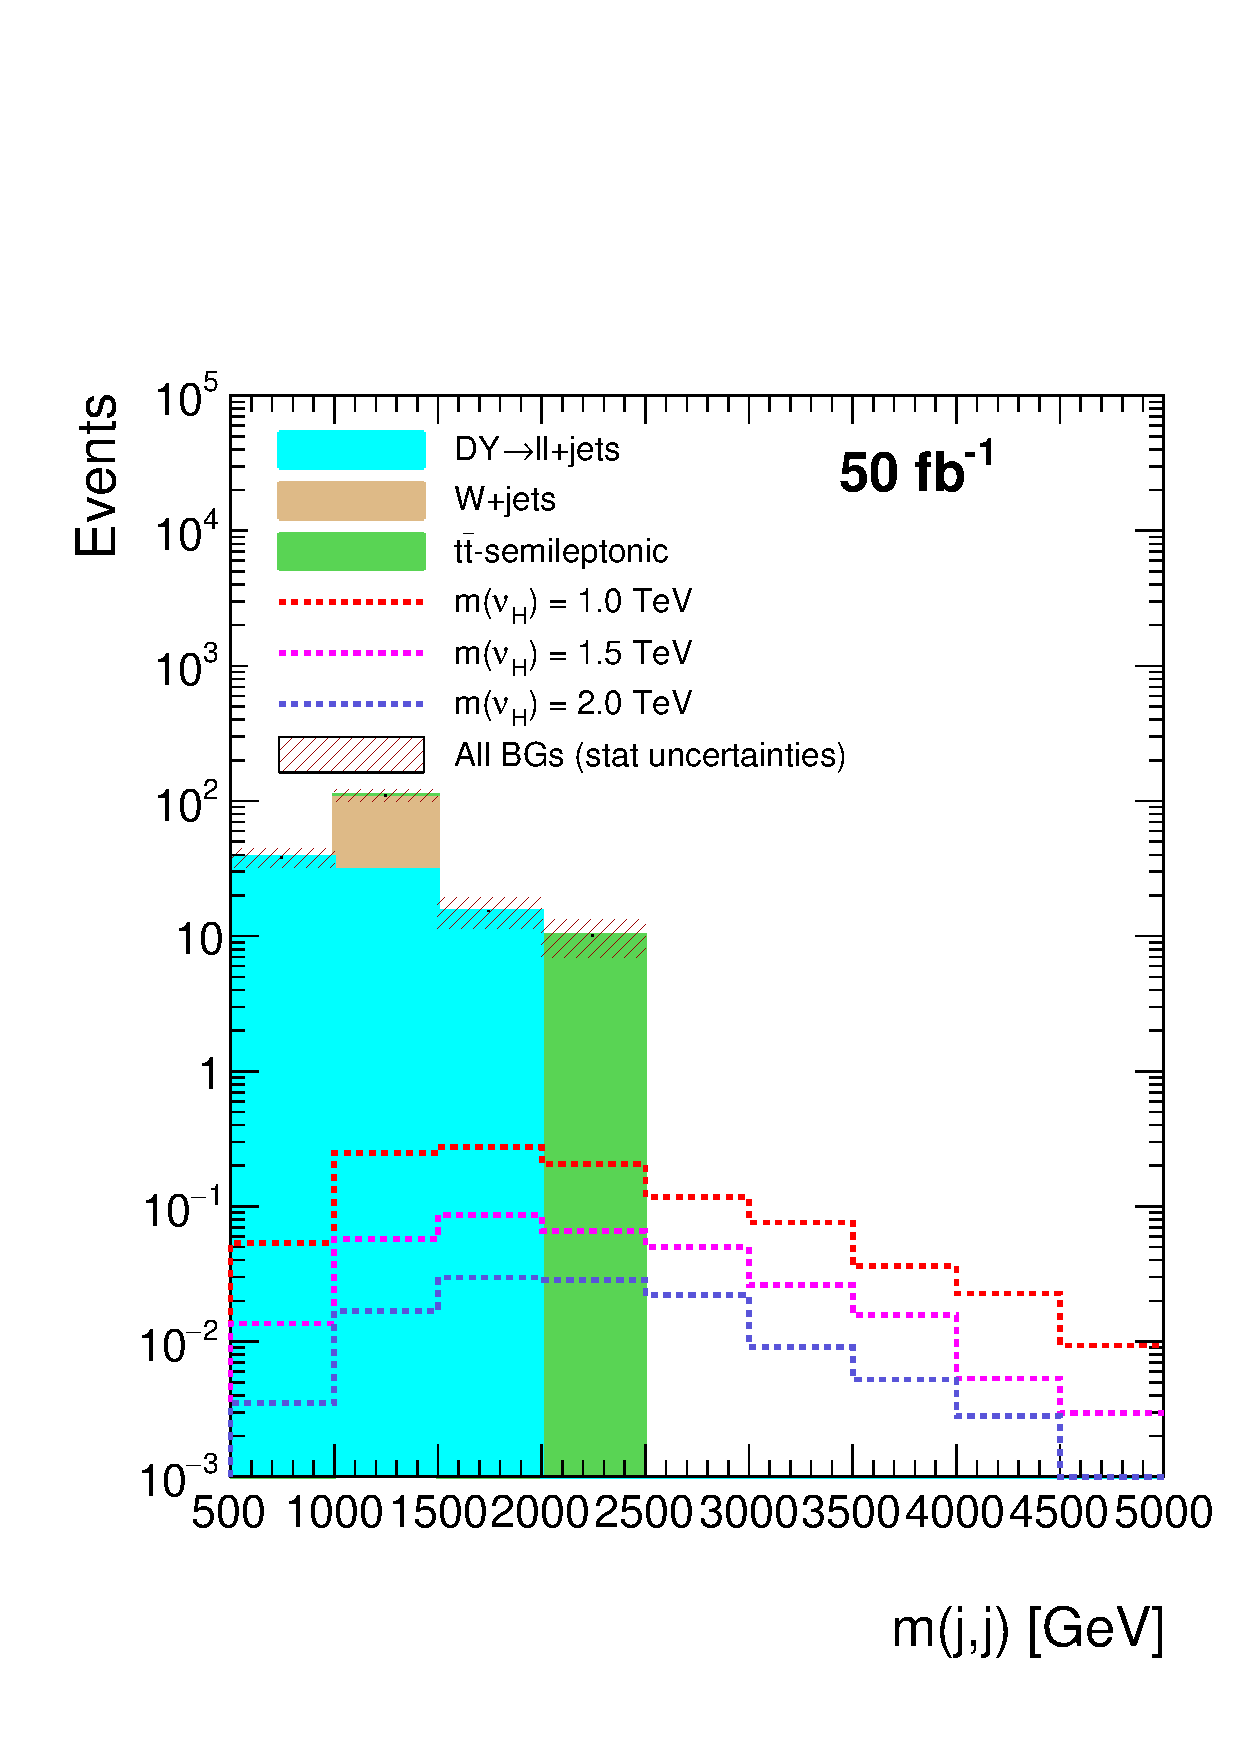
\includegraphics[width=\linewidth]{StackPlots/mjj_2taus_met50_50ifb.pdf}
\caption{Stack plot of Di-Jet mass requiring two taus in the event and with $\slashed{E}_{T} > 50$}
\label{fig: mjj2tausMet50}
\end{figure}

\begin{figure}[H]
\centering
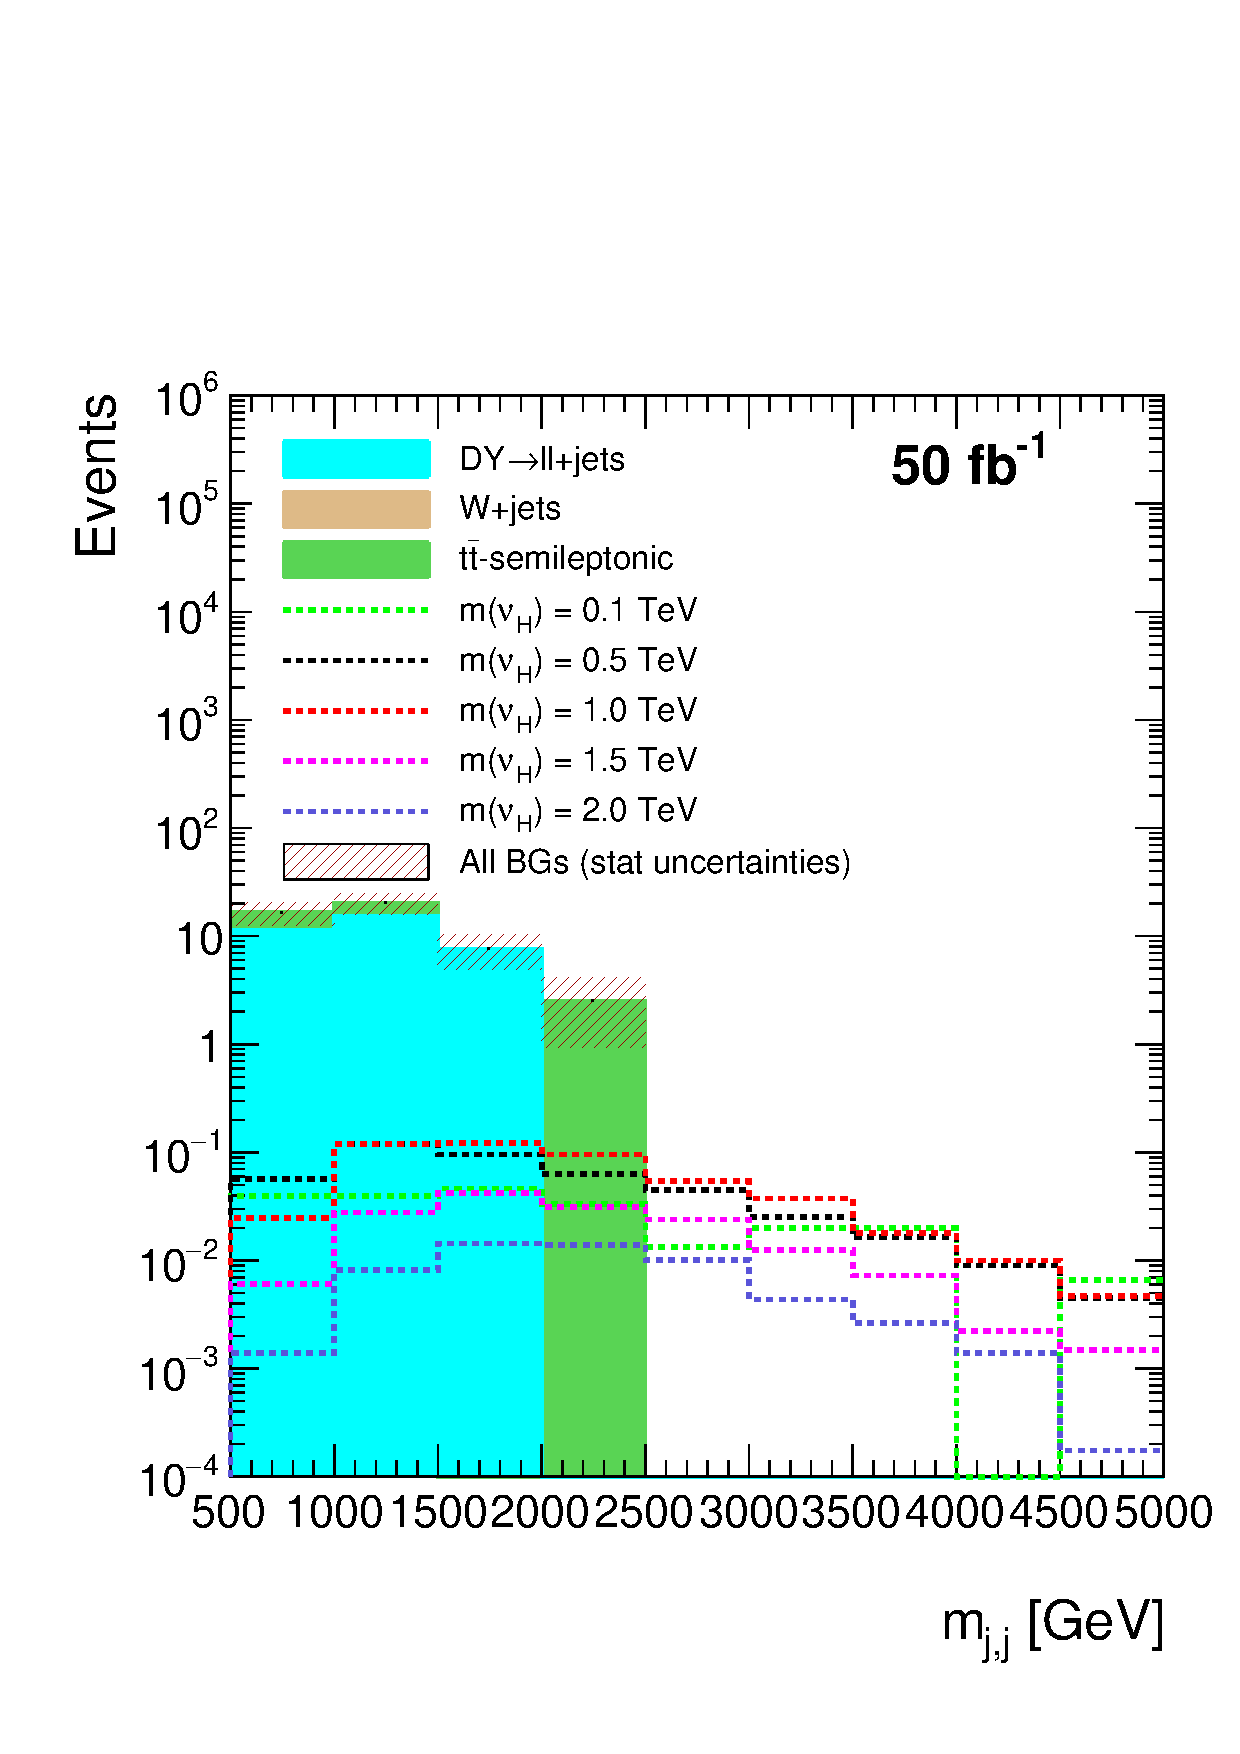
\includegraphics[width=\linewidth]{StackPlots/mjj_2Taus_met60_50ifb_2moreSignals.pdf}
\caption{Stack plot of Di-Jet mass requiring two taus in the event and with $\slashed{E}_{T} > 60$}
\label{fig: mjj2tauMet60}
\end{figure}

\begin{figure}[H]
\centering
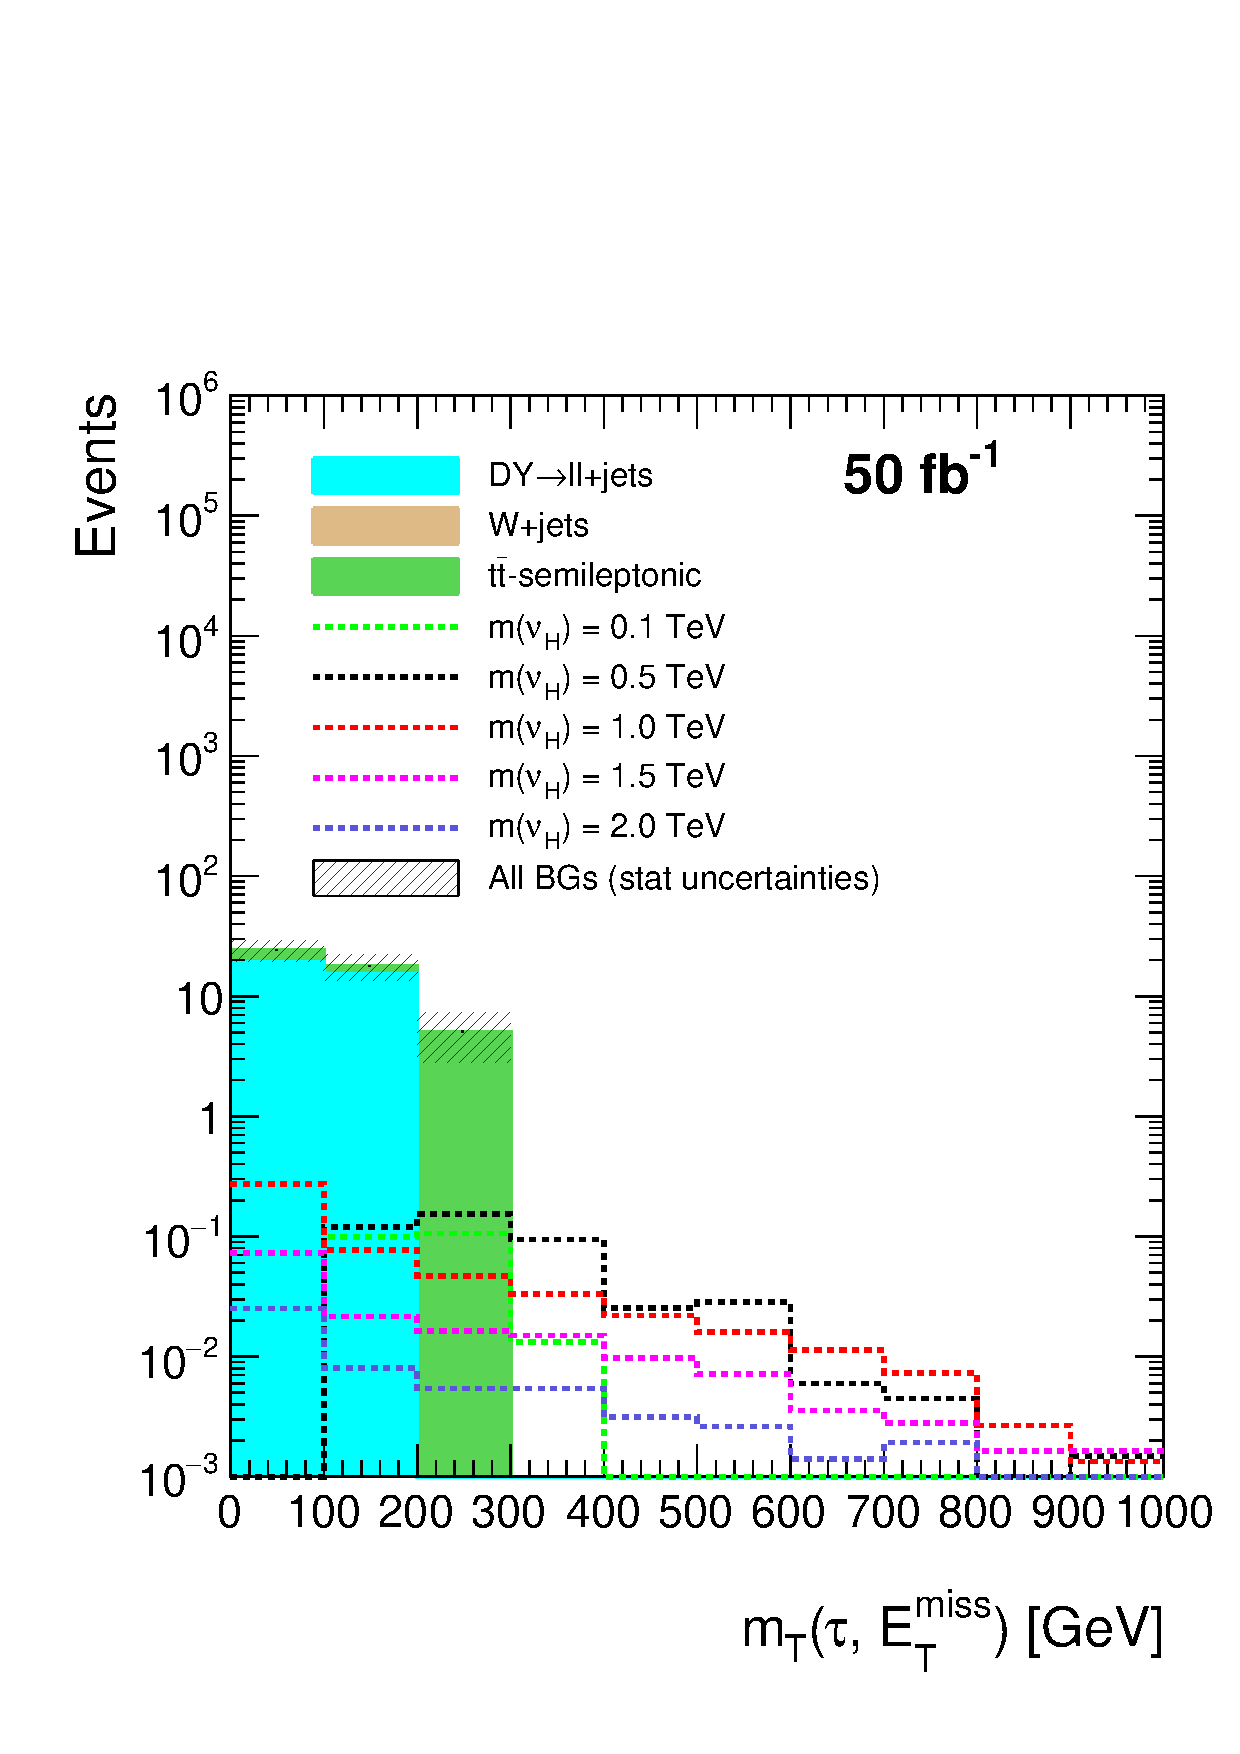
\includegraphics[width=\linewidth]{StackPlots/mT_2Tau_met60_50ifb_2moreSignals.pdf}
\caption{Stack plot $m_{T}$ between the $\tau$ and the $\slashed{E}_{T}$ requiring two taus in the event and with $\slashed{E}_{T} > 60$}
\label{fig: mT2tausMet60}
\end{figure}



Besides the case requiring two taus in the event with the selection criteria mentioned previously, the case requiring only one tau with a minimum transverse momentum of 50 GeV was studied. The plots for this case are shown in Figures \ref{fig: MET1tauMet60}, \ref{fig: mjj1tauMet60}, and \ref{fig: mT1tauMet60}. These three plots already include the increase in the $\slashed{E}_{T}$ cut discussed at the beginning of this section. In these plots it can be seen that the total amount of background for this case is increased in almost three orders of magnitude. In particular, the W+jets process has significantly more events in the case for one tau after applying all the cuts. However, the dominant background process for both the two taus and one tau cases is the Drell-Yan process. 

The main difference between the one tau and two tau case in the relevance of the Di-Jet mass variable. As mentioned earlier, the amount of background increases significantly for the case where only one tau in the event is required. This amount in the background affects the separation between signal and backgrounds in $m(jj)$ observed in the case where two taus were required. This fact can be seen in the Di-Jet mass distribution presented in \ref{fig: mjj1tauMet60}. This is why the distribution of the transverse mass between the tau and the missing transverse energy was explored. Figure \ref{fig: mT1tauMet60} shows the distribution of $m_{T}$ for the case of requiring only one tau. It can be observed that, although a separation as good as the one obtained in $m(jj)$ for the two taus case, the $m_{T}$ distribution has a greater separation between signal and backgrounds than the one in $m(jj)$ in Figure \ref{fig: mjj1tauMet60}.


\begin{figure}[H]
\centering
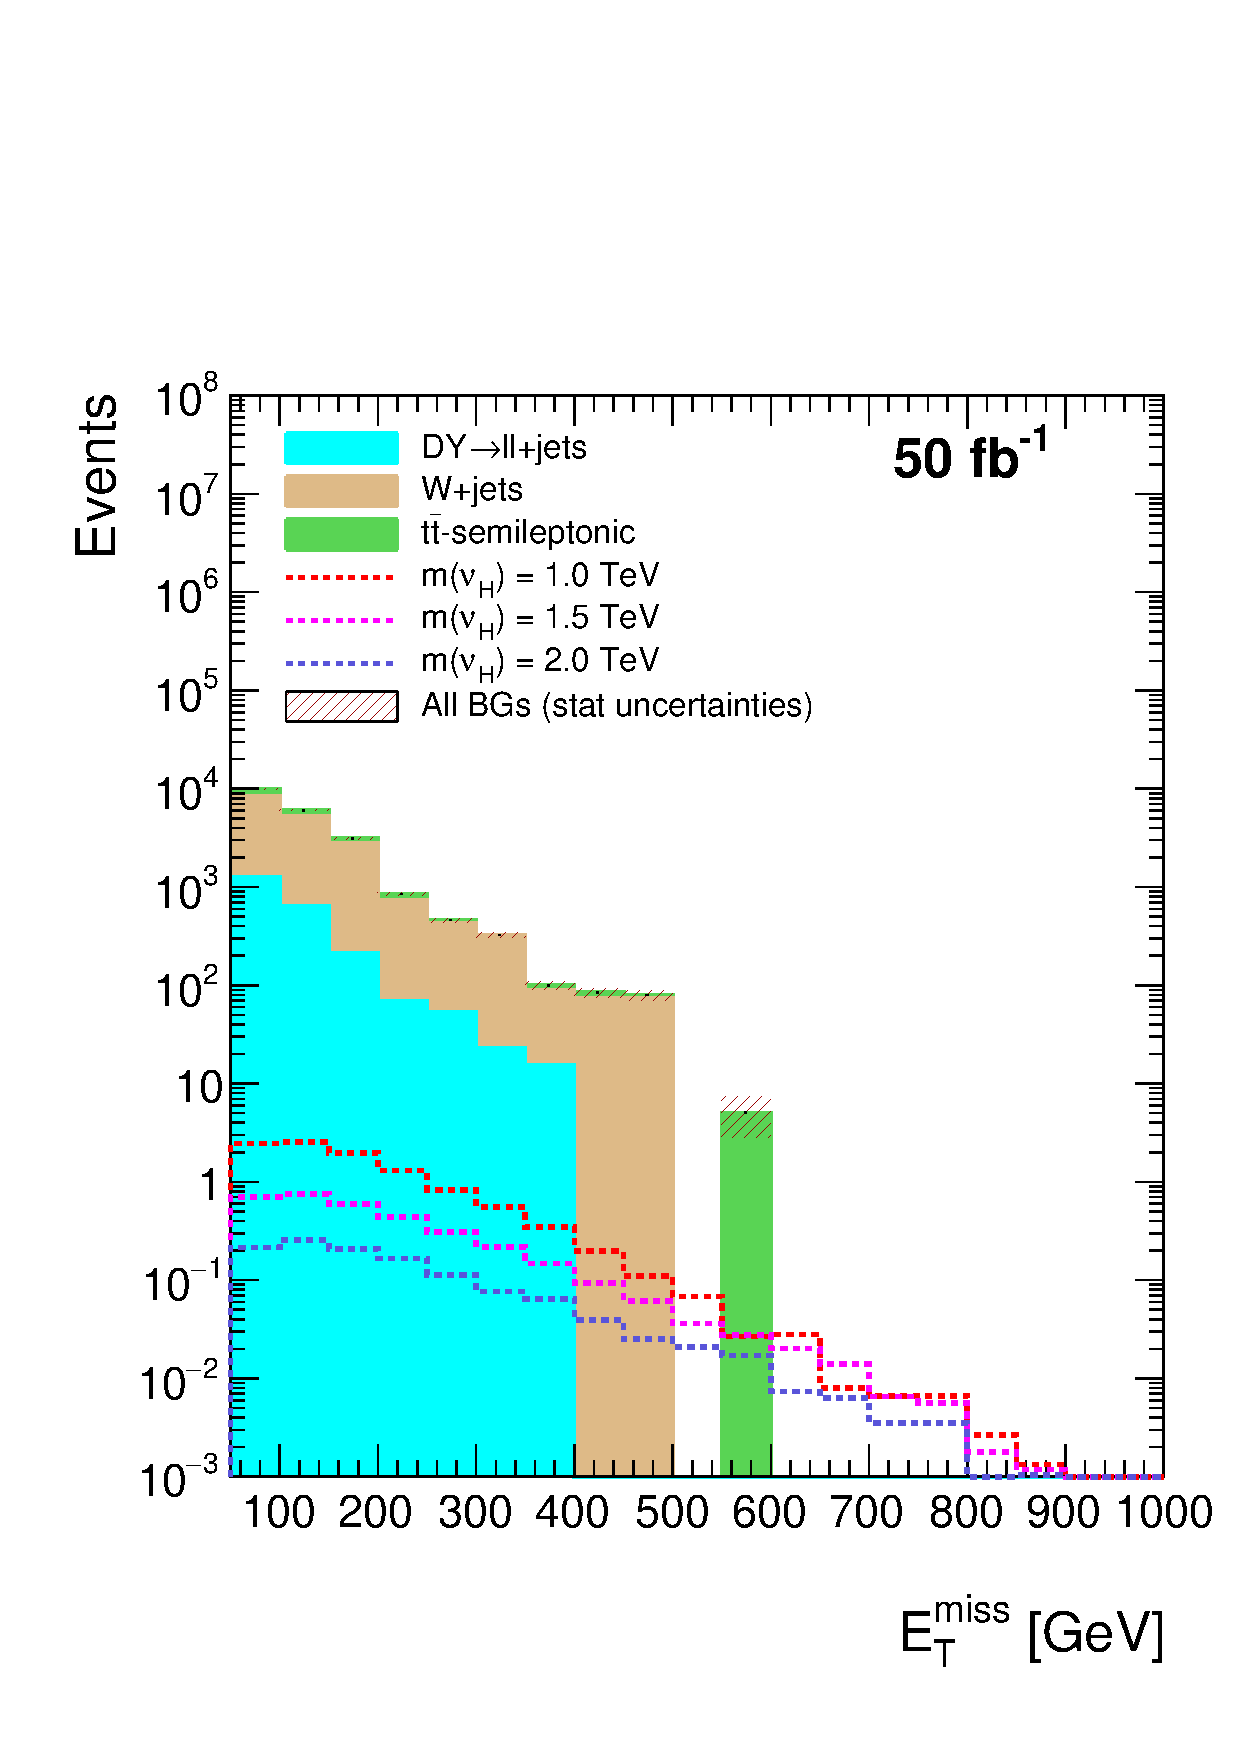
\includegraphics[width=\linewidth]{StackPlots/MET_1Tau_met60_50ifb.pdf}
\caption{Stack plot of $\slashed{E}_{T}$ requiring one tau in the event and with $\slashed{E}_{T} > 60$}
\label{fig: MET1tauMet60}
\end{figure}

\begin{figure}[H]
\centering
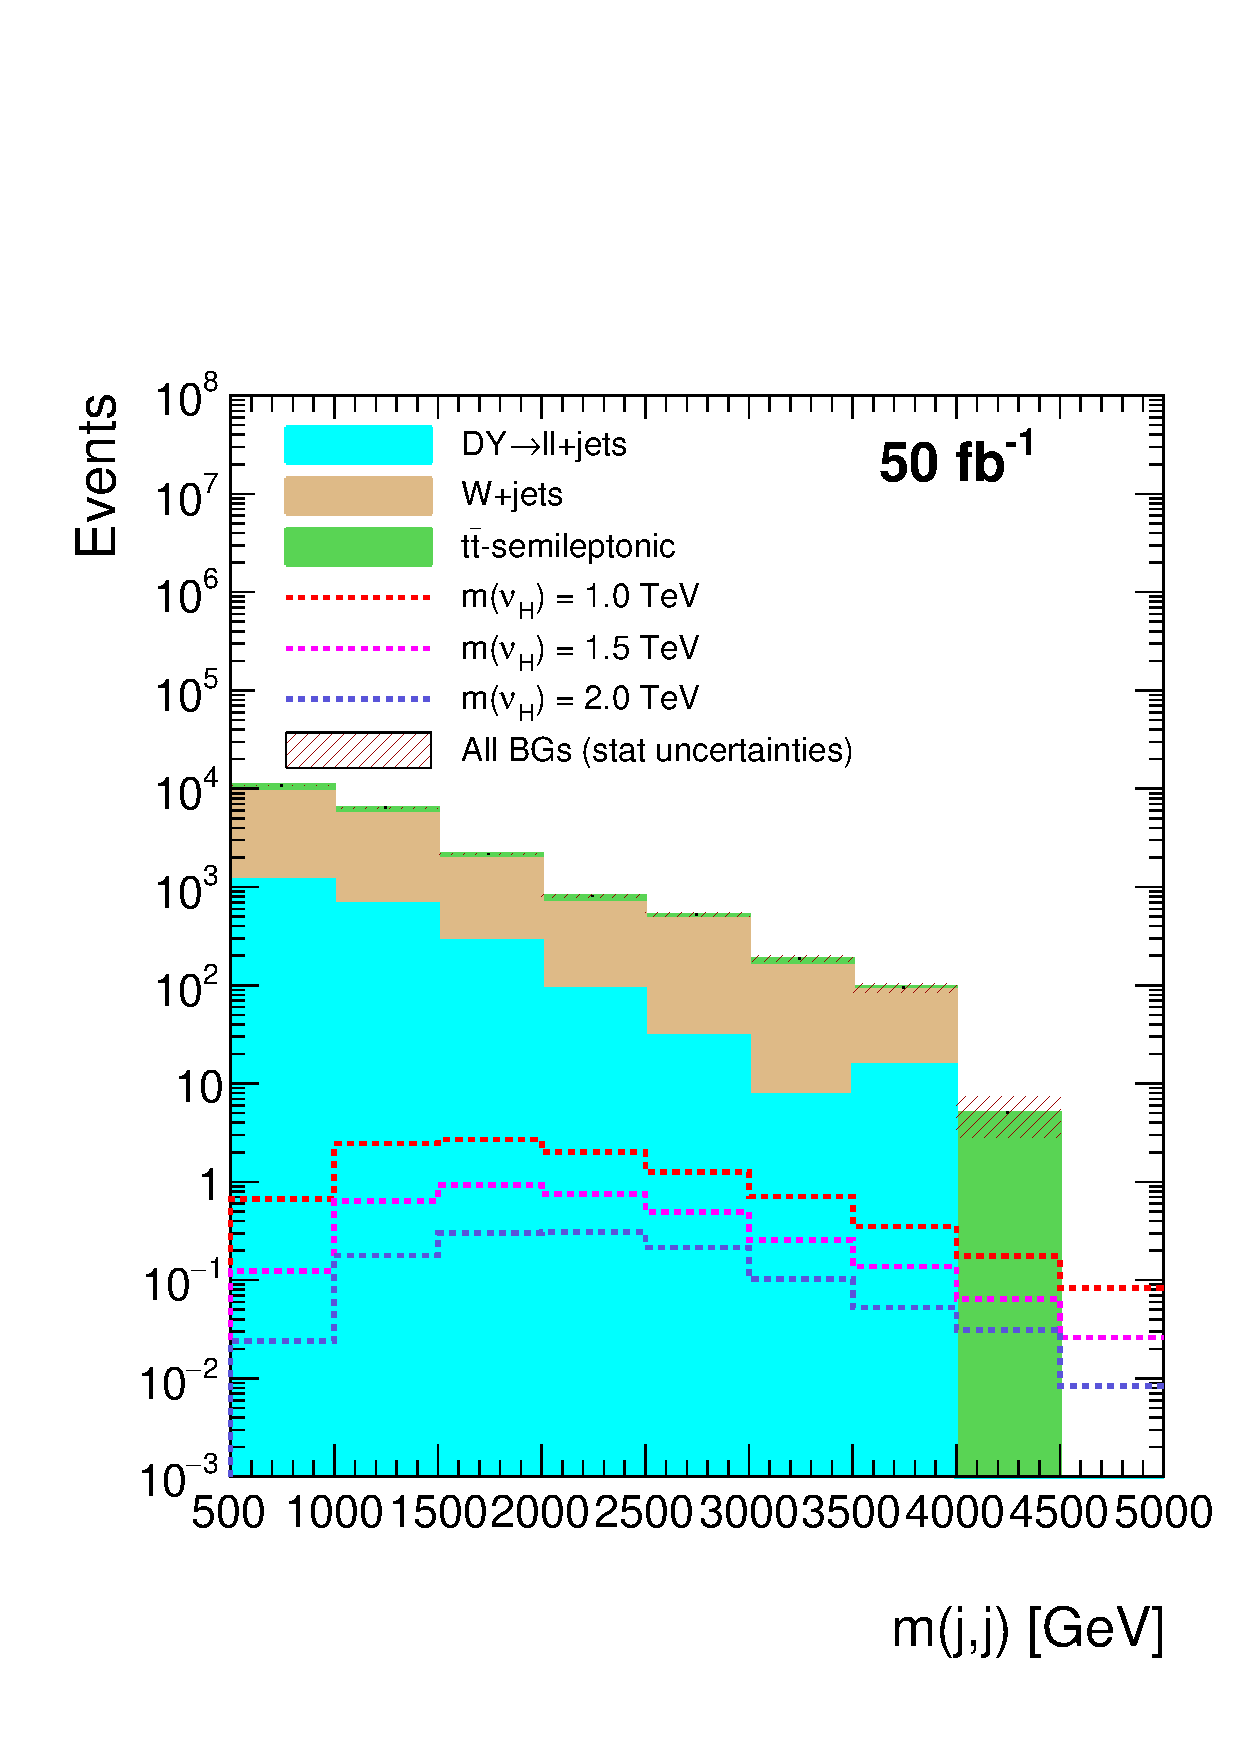
\includegraphics[width=\linewidth]{StackPlots/mjj_1Tau_met60_50ifb.pdf}
\caption{Stack plot of Di-Jet mass requiring only one tau in the event and with $\slashed{E}_{T} > 60$}
\label{fig: mjj1tauMet60}
\end{figure}




\begin{figure}[H]
\centering
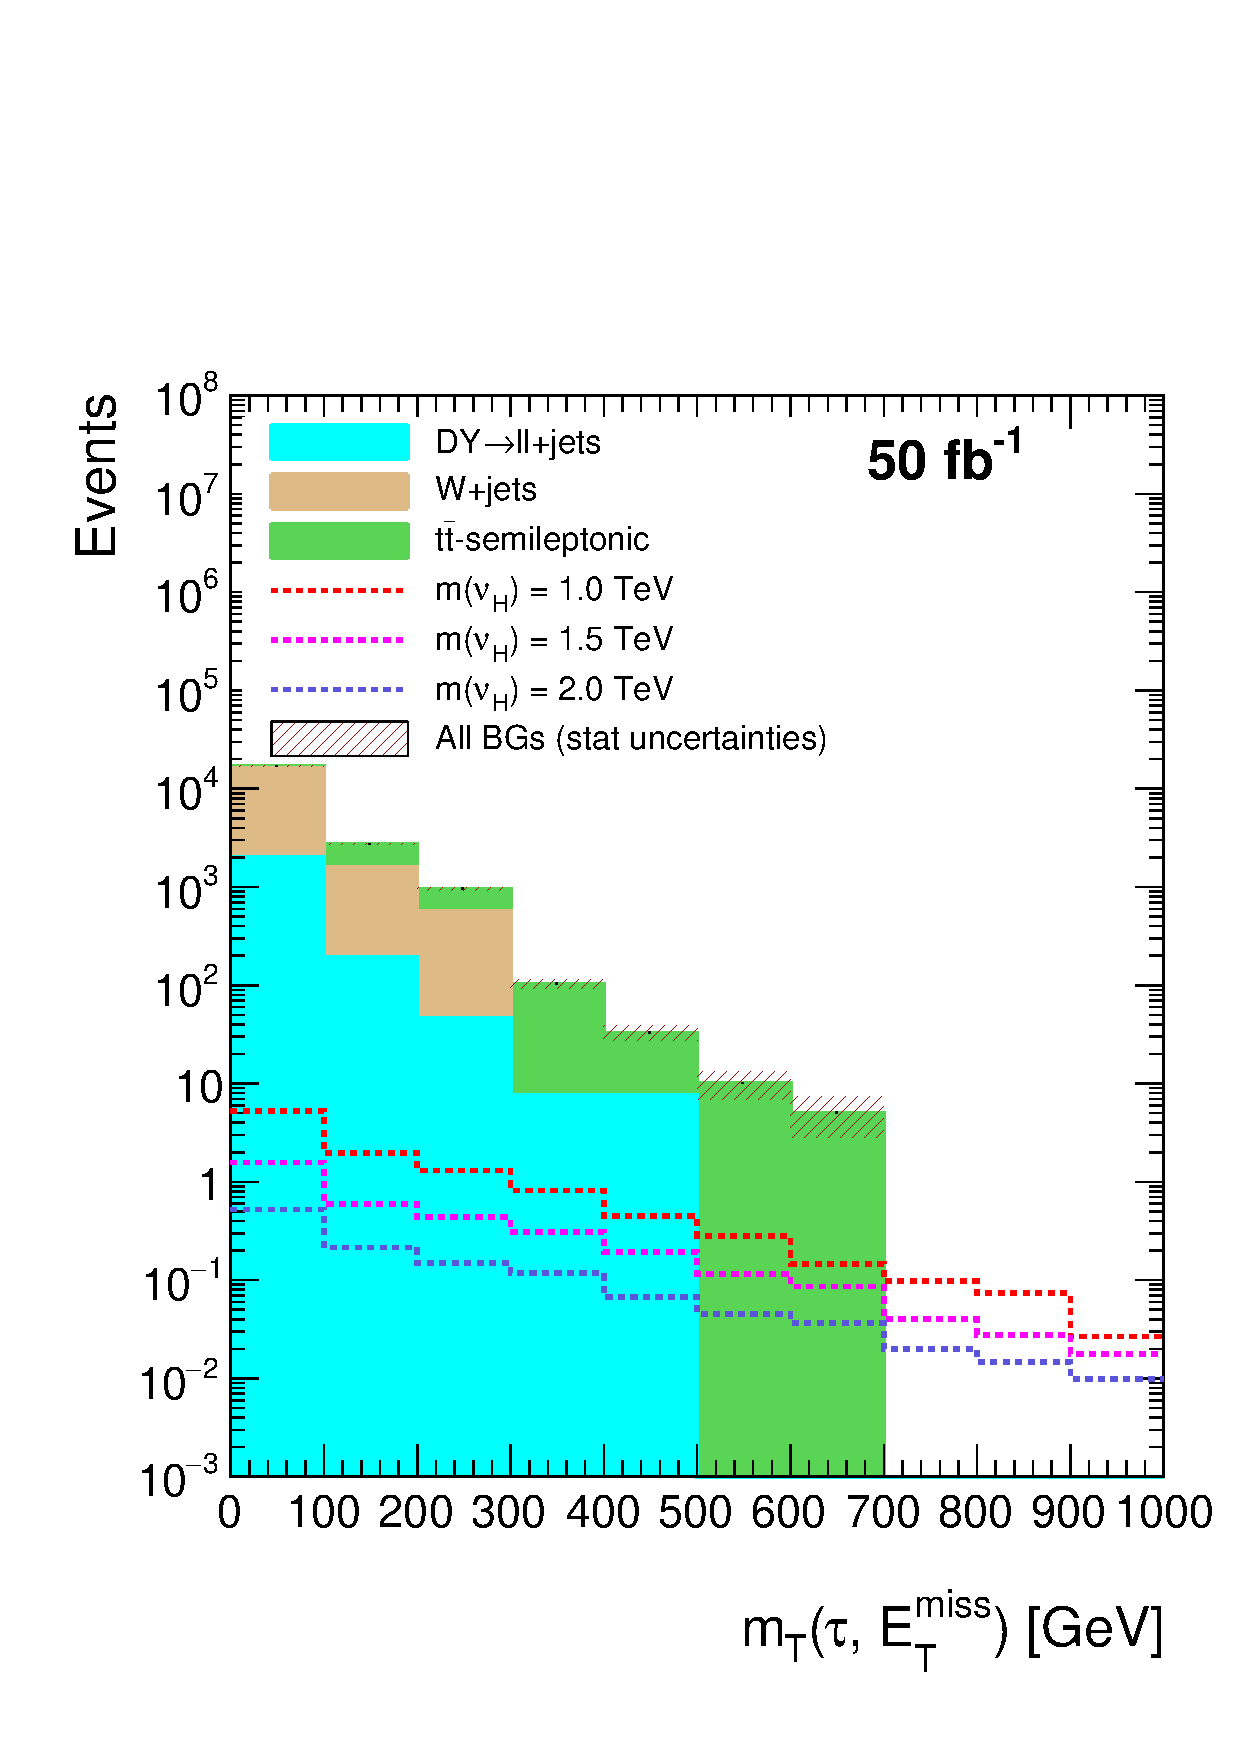
\includegraphics[width=\linewidth]{StackPlots/mT_1Tau_met60_50ifb.pdf}
\caption{Stack plot $m_{T}$ between the $\tau$ and the $\slashed{E}_{T}$ requiring only one tau in the event and with $\slashed{E}_{T} > 60$}
\label{fig: mT1tauMet60}
\end{figure}










